\documentclass{book}

\addtolength{\textwidth}{3cm}  \addtolength{\oddsidemargin}{-1.5cm}  \addtolength{\evensidemargin}{-1.5cm}
\addtolength{\textheight}{1cm} \addtolength{\topmargin}{-.3cm}

\usepackage{amssymb}
\usepackage{amsmath,bm}

\usepackage{booktabs}
\usepackage{aicescover}
\usepackage{hyperref}
\hypersetup{
    colorlinks=false, %set true if you want colored links
    linktoc=all,     %set to all if you want both sections and subsections linked
    linkcolor=blue,  %choose some color if you want links to stand out
}

\usepackage[
backend=bibtex8,
sorting=ynt,
maxbibnames=99
]{biblatex}
\addbibresource{bibliography.bib}

\linespread{1.1}
\pagestyle{plain}
\usepackage{graphicx}
\usepackage{caption}
\usepackage{subcaption}
\usepackage{enumitem}
\usepackage{placeins}
%\usepackage{algorithm}
\usepackage{algorithm}
\usepackage{algpseudocode}
\usepackage{glossaries}
\usepackage{appendix}
\usepackage{xr}
\usepackage{color}
\usepackage{longtable}
\DeclareMathOperator*{\argmin}{arg\,min} % Jan Hlavacek
\newcommand\norm[1]{\left\lVert#1\right\rVert}


\makeglossaries
\loadglsentries{glossary.tex}

\graphicspath{ {Figures/} }

\begin{document}

\aicescovertitle{Analyses of Convolutional Neural Networks for Automatic tagging of music tracks }
\aicescoverauthor{{\bf Master Thesis}\\by\\Aravind Sankaran\\ \\May 2017}
\aicescoversupervisor{Prof. Paolo Bientinesi \\ Prof. Marco Alunno}
\aicescoverexaminer{Prof. Paolo Bientinesi \\ Prof. Bastian Leibe}
\aicescoverpage


\section*{Abstract}

Describing music can be quite tricky and talking about music may simply require as much vocabulary as any technical subject. This makes analysing music and communicating it's musical syntax challenging. An algorithm that  automate the task of attaching a semantic description to a song should extract relevant features from the audio signal for optimum performance.
Supervised feature learning is used to obtain features that could be optimum for our context of music tagging. Convolution Neural Networks(CNN) and Sequence to One Long-Short Term Memory(LSTM) Recurrent neural networks are used to induct supervised learning into the feature extraction pipeline. A repertoire of 842 songs with carefully labelled data is used for training. Since our target dataset is small, the model is first trained on \textit{MagnaTagATune}(MTT) public dataset. The performance of transfer learning with CNN and LSTM are compared for different levels of supervised fine-tuning in the feature extraction pipeline and the Weighted averaged Area Under receiver operating characteristic Curve (WAUC) scores are reported. It has been found that the performance of CNN and LSTM, when fine-tuned on target dataset, is better than the corresponding models trained on MTT dataset used as black-box feature extractors for target task. These models are also compared with Mel-Frequency-Cepstral-coefficient(MFCC) features approximated by Bag of Frames algorithm which does not require labelled data. The performance with features extracted by fine-tuned CNN is lesser than MFCCs for our target task.   
  

\vspace{5cm}


\newpage

\section*{\bf Acknowledgments}
I would like to thank \textit{Prof. Paolo Bientinesi} (High performance and automatic computing group, AICES, RWTH Aachen) for doing one of the most expensive work - \textit{Listen to the songs and tag them}. I also thank  \textit{Prof. Marco Alunno} (Professor of Composition and Theory at University EAFIT, Columbia) for his valuable association and advices.  
\tableofcontents

% Chapter 1
\externaldocument{chapter3}
\externaldocument{chapter4}
\chapter{Introduction} % Main chapter title

\label{Chapter1} % For referencing the chapter elsewhere, use \ref{Chapter1} 

%----------------------------------------------------------------------------------------

% Define some commands to keep the formatting separated from the content 
\newcommand{\keyword}[1]{\textbf{#1}}
\newcommand{\tabhead}[1]{\textbf{#1}}
\newcommand{\code}[1]{\texttt{#1}}
\newcommand{\file}[1]{\texttt{\bfseries#1}}
\newcommand{\option}[1]{\texttt{\itshape#1}}

%----------------------------------------------------------------------------------------

%\section{Welcome and Thank You}

Computers have been used to automate discovery and management of music in so many different ways. Automating the task of attaching a semantic meaning to a song is popularly known as \textit{music auto-tagging}. Automatic tagging algorithms have been used to build recommendation systems that allow listeners to discover songs that match their taste. But semantic description of a song is not straightforward and there is this gap between music audio and listener's description. In section \ref{motivation}, the need for this dedicated research is explained by describing some shortcomings of the currently available solution approaches. In section \ref{overview}, an overview of the contents of this research is presented.   

%----------------------------------------------------------------------------------------

\section{Motivation}
\label{motivation}
Developing an algorithm that imitates the human way of describing auditory scene is an interesting application. Although great technical progress have been made to enable efficient retrieval and organization of audio content, analysing music and communicating it's musical syntax that respects multidimensional qualities of sound is still challenging. Current music recommendation systems fall short in providing recommendations by respecting the criteria emerging from perceptual qualities of music because of the reasons described below,
  
\subsection{Challenges with collaborative filtering methods}
When the usage data is available, one can use collaborative filtering to recommend the tracks on a community-based trending lists (say, a community of experts). That is, if a listener liked songs A and B and you liked A, you might also like B. Such algorithms have proven to be extremely efficient and out-perform those algorithms that works by extracting acoustic cues from audio signal for the task of finding similar songs \cite{DC1}. However, in absence of such usage data, one resorts to content-based methods, where just the audio signal is used for generating recommendations. Thus collaborative filtering methods suffer from what is called a \textit{cold start problem}, making it less efficient for new and unpopular songs. 


\subsection{Challenges with content based methods}
\label{problems}
Using information from audio content to overcome the cold-start problem resulted in \textit{content-based} recommendation methods. In such algorithms, acoustic cues required for discriminating the semantics are extracted from the audio signal. These acoustic cues have to be encoded in the lower dimensional approximation of audio signal, also known as features. However, to provide descriptions that could come closer to human intelligence, the features should also encode the perceptual information in the song. The current state-of-art content based music tagging algorithms\cite{MultiScale}\cite{choi_crnn} use large sets of data to train an algorithm to automatically detect the optimal features from a spectrogram representation of the audio signal. This kind of training is known as \textit{feature learning}. Unsupervised learning (training data is not labelled) used in \cite{MultiScale} may not extract features that would be optimal for all contexts of music tagging. Supervised learning used in \cite{choi_crnn}\cite{choi_cnn} can extract features optimal for context used, but need large amount of labelled data for training.      


%----------------------------------------------------------------------------------------

\section{Overview}
\label{overview}
Convolution neural networks (CNN) have recently gained popularity for content-based multi-label classification task achieving state-of-art performance\cite{choi_cnn}\cite{choi_crnn} on established datasets\cite{MSD}\cite{MTT}. But these models were trained on large amount of labelled training data containing short excerpts of music of fixed size (29.1s). The aim of this thesis is to find out
\begin{itemize}
\setlength\itemsep{0em}
\item If the CNN models trained on large data can be exploited to show similar performance gains with \textit{transfer-learning} on smaller dataset. That is, the CNN is first trained on a large labelled dataset and the converged weights are used as initialization for training on smaller dataset. 
\item Models that can extract features by approximating signals of arbitrary length.
\end{itemize} 
    
\noindent For the purpose of analysing feature learning, the feature extraction pipeline for music information retrieval is formalised into following stages: \textit{signal representation}, systematic \textit{dimensionality-reduction} followed by \textit{temporal approximation}.
  
\subsection{Signal Representation}
Music is distinguished by the presence of many relationships that can be treated mathematically by analysing the frequency content. Motivated by the way ear-brain handles the frequency information, myriad of features extracted from spectrogram representations were evolved. In this thesis, following the analyses from current literature \cite{choi_cnn}\cite{EndToEnd}\cite{MultiScale}\cite{choi_crnn}, only \textit{mel-spectrogram} representation is used. \textit{Mel-spectrograms} exploit the fact that our ear cannot distinguish adjacent frequencies (say, we cannot differentiate 300 KHz and 310 KHz), and the frequencies values are binned according to a what to popularly known as \textit{mel-scale}. In chapter 2, section \ref{time}, representation of digital audio in time-frequency format is explained. In section \ref{stft}, computations of mel-spectrogram as a convolution operation is elaborated.
   
\subsection{Dimensionality reduction}
The signal representation is divided into short frames and the dimension of each frame is reduced systematically by discarding information that does not contribute to discrimination. The mathematical operators that discard information not contributing to variance in our context specific classification task can be obtained by solving for parameters of CNNs. In chapter 2, section \ref{stacked}, formalism of CNN as feature extractor for MIR tasks have been illustrated and in section \ref{training}, challenges in training CNN have been pointed out. The training dataset for our thesis (target dataset) is small. Therefore CNN is first trained on the publicly available \textit{MagnaTagATune} dataset\cite{MTT} and \textit{transfer-learning} on our target dataset is comparatively analysed in chapter 4, section \ref{cnn_s}.

\subsection{Temporal approximation}
The reduced information from each frame are temporally approximated to a fixed sized representation. The classifier then takes these fixed sized features and outputs the tags. The resulting approximation should not lose the perceptual information required for discrimination. To do this, supervised learning with \textit{sequence to one} Recurrent Neural Network (RNN) is used, that sequentially combines reductions from each frame to a fixed size feature. Formalisms of RNN are presented in chapter 2, section \ref{rnn} and comparative analyses of transfer learning with CNN + RNN models are discussed in chapter 4, section \ref{cnn_s} 
  
%----------------------------------------------------------------------------------------

\section{Outline of the report}
In chapter 2, the fundamentals of mathematical concepts used in this thesis are explained and formalism of notations are introduced. In chapter 3, a detailed overview of previous research and justification for our proposed models for analyses are discussed. In chapter 4, details of the datasets, evaluation metrics, parameter settings and the experiment results are analysed. In chapter 5, the inference from these experiments and future directions are proposed. 







% Chapter 2

\externaldocument{chapter3}
\externaldocument{chapter4}
\externaldocument{chapter5}
\externaldocument{chapter1}
\externaldocument{AppendixA}
\chapter{Formalisms} % Main chapter title

\label{Chapter2} % For referencing the chapter elsewhere, use \ref{Chapter2} 


%----------------------------------------------------------------------------------------

%\section{Welcome and Thank You}
%In this chapter, acoustical characteristics of music signal that enables general MIR tasks will be introduced.We will examine the Fourier Series representations of sound waves and see how they relate to harmonics and tonal color of instruments  
To map a music to it's semantic descriptions, the signal is first transformed to a lower dimensional space. The resulting transformation is called \textit{feature}. The classifier then takes these features as input and performs the classification task. The performance of the classifier can only be as good as the information encoded in the features. In this chapter, formalisms required for the analysis of feature extraction are introduced. The raw signal is first changed to a representation that can be mathematically analysed (see Sec. \ref{rep}). This representation is then transformed to a lower dimensional space by discarding information that does not contribute to discrimination (see Sec. \ref{dimension}). The resulting reduction is then approximated to a fixed size representation (see Sec. \ref{temporal}) which is then taken as input by a multi-label classifier (see Sec. \ref{classifier}). In section \ref{training}, training procedure that can optimize feature representations for supervised classification task is discussed. 
%----------------------------------------------------------------------------------------

\section{Representation of music signal}
\label{rep}
The observed signal is traditionally represented in the time domain. The time domain is a record of what happened to a parameter of the system versus time. Standard formats use amplitude versus time. The observed signal is then discretised by sampling and stored in digital format (see \ref{sampling}). This signal in the time domain is then changed to frequency domain (see \ref{time}). This is simply because our ear-brain combination is an excellent frequency domain analyser. Currently used music signal representations for general MIR tasks are explained in section \ref{stft}.


\subsection{Sampling of continuous-time signal}
\label{sampling}
The digital formats contain the discrete version of the signal obtained by sampling continuous-time signal. Sampling is performed by measuring the value of the continuous signal every $T$ seconds. This interval $T$ is called the sampling interval or the sampling period. The sampling frequency or sampling rate ($f_{s}$) is the number of samples obtained in one second (samples per second),  
\[
 f_{s} = \frac{1}{T}.
\]
The optimum sampling rate is given by Nyquist-Shannon sampling theorem which says, the sampling frequency $f_{s}$ should be at least twice the highest frequency contained in the signal. Given the human hearing range lies between 20Hz - 20KHz, most of the digital audio formats use a standard sampling frequency of 44.4Khz. Sampling rate determines the initial dimension of the raw signal. The signal may be further down sampled if higher sampling rate does not contribute to classification performance.

\subsection{Time-Frequency transformations}
\label{time}
The digital signal is represented in the time domain with amplitude values at each time $t$. This representation has to be changed to frequency domain. Mapping from time-domain to frequency-domain is looked up on as basis transformation. 

\subsubsection{Basis transformation from time to frequency domain}
\noindent The signal in the time domain $\textbf{a}$ is a set of ordered \textit{n}-tuples of real numbers \( (a_{1},a_{2}, ...,a_{N}) \in \mathbb{R}^N \) in the vector space \textit{V}, specifically \textit{Euclidean n-space}. That is to say, a discrete-time signal can be represented as a linear combination of Cartesian basis vectors. The coefficients in linear combination are then the co-ordinates of the corresponding basis system.  
\[
\textbf{a} = (a_{1},a_{2}, ...,a_{N}) = a_{1}\textbf{e}_{1} + a_{2}\textbf{e}_{2} + ... + a_{N}\textbf{e}_{N} = \displaystyle\sum_{t=1}^{N}a_{t}\textbf{e}_{t} = \mathbb{I}\textbf{a}
\]
Where $(a_{1},a_{2}, ...,a_{N})$ are the co-ordinates of Cartesian basis formed by basis vectors $\textbf{e}_{1} ... \textbf{e}_{N}$ with $t \in \{1,2,..N\}$. The unit vector $\textbf{e}_{t} \in \mathbb{R}^{N}$ has 1 in the $t^{th}$ index and 0 everywhere else.
\bigskip

\noindent To transform to frequency domain, we need to find a set of basis vectors $\bm{\phi}_{ \omega }$ that are functions of frequencies ($\omega$). Then the co-ordinates of this basis system $c_{ \omega }$ represents the signal in frequency domain. 
\begin{equation}
\label{exp_fourier}
\textbf{a} = \displaystyle\sum_{ \omega =1}^{M}c_{ \omega }\bm{\phi}_{ \omega } = \bm{\Phi}\textbf{c} \qquad \bm{\Phi} \in \mathbb{C}^{N \times M}, \textbf{c} \in \mathbb{C}^{M}
\end{equation}
If $\bm{\Phi}$ is known, then the transformed co-ordinates $\textbf{c} = (c_{1},c_{2},..,c_{M})$ can be computed as,
\[
\textbf{c} = \bm{\Phi}^{-1}\textbf{a}
\]
$\textbf{c}$ is the transformed representation. $\bm{\Phi}^{-1}$ is the operator that transforms the signal. 

\subsubsection{Exponential Fourier Series and Fourier Transform}
From the definition of \textit{exponential Fourier Series}, any function \textit{periodic} in $\{1,2,..,T\}$ can be expanded with series of complex exponentials\cite{allen}. These complex exponentials which are functions of harmonically related frequencies($k \omega$) form basis 
\[
\bm{\phi}_{k}(t) = \frac{1}{\sqrt{T}}e^{ik \omega t} \qquad t \in \{1,2,..T\}
\] 
It is difficult to assume periodicity for a generalized signal. Hence, the Fourier series can not be applied directly and Fourier Transform was developed. By Fourier transform, quantity of each frequency component $\omega$ in an arbitrary signal $\textbf{a}(t)$ can be computed by dividing by $e^{i \omega t}$. Application of Fourier transform to a discrete signal is called \textit{Discrete Fourier Transform}
\[
c_{\omega} =  \displaystyle\sum_{t=1}^{N}a_{t}e^{-i \omega t} \qquad t \in \{1,2,...,N\}
\] 
Thus the transformation operator is,
\[
\bm{\Phi}^{-1}[ \omega ] = e^{-i \omega \textbf{t}} \qquad \textbf{t} \in \mathbb{R}^{N}, \omega \in \{1,2,..,M\}
\]
Fast Fourier Transform(FFT) is an efficient implementation of Discrete Fourier Transform(DFT) which exploits the symmetry of $sines$ and $cosines$ in the complex exponential. While DFT requires $O(N^2)$ operations, FFT requires only $O(NlogN)$ \cite{allen}. 


\subsection{STFT, Mel-Spectrogram}
\label{stft}
It is useful to perform FFT locally over short segments. This is because we are more interested in the evolution of frequency content rather than the frequency content of the entire signal. Hence, the full length signal is divided into short segments, and FFT is computed separately for each segment. This is known as \textbf{Short Time Fourier Transform (STFT)}. One common problem with STFT is the \textit{spectral leakage}, which is addressed by modifying the original signal with some window function. The most common window function is the \textbf{Hamming Window} defined as,
\begin{equation}
h[n] = 0.54 - 0.46cos(\frac{2 \pi n}{N-1})
\end{equation}
where $n \in \{1,2,..,F\}$ and $F$ is the size of window function. The signal approaches zero near $n=1$ and $n=N$, but reaches peak near $n=N/2$ \cite{specLeak}. To overcome the information loss at the ends of the window, signal is divided into segments that are partly \textit{overlapping} with each other. The distance between the start of two adjacent segments is called \textit{hop-length}. Figure \ref{fig:stftPipe} shows the extraction of spectral frames of a spectrogram. Thus, the parameters of STFT include 
\begin{itemize}
    \setlength\itemsep{0em}
    \item Choice of window function
    \item Size of each segment in $\textbf{a}$ ($F$)
    \item Hop length or stride ($s$) of the transformation operator
    \item Size of frequency dimension $M$ (also known as FFT size)
\end{itemize}

\begin{figure}[h]
       \begin{subfigure}[b]{0.6\textwidth}
        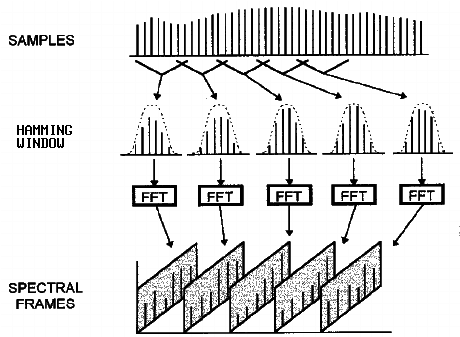
\includegraphics[width=\textwidth]{stft_pipe}
        \caption{Windowing is applied on overlapping segments\\ followed by FFT }
        \label{fig:stftPipe}
       \end{subfigure}
	    \begin{subfigure}[b]{0.4\textwidth}
        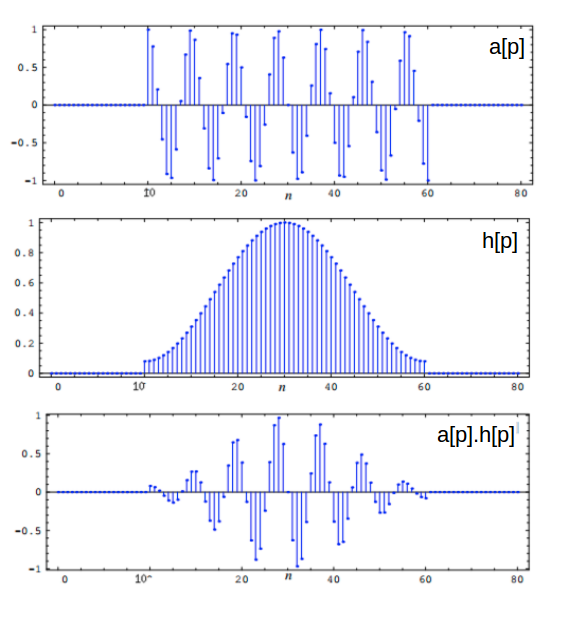
\includegraphics[width=\textwidth]{stft}
        \caption{
        Application of Hamming Window on \\a segment of input signal
        }
        \label{fig:HammingWindow}
       \end{subfigure}
       \caption{\cite{spec_dia} (a) Shows STFT Pipeline. (b) Shows the application of \\Window function}\label{fig:STFT}
\end{figure}
\FloatBarrier

\subsubsection{STFT as Convolution}
\noindent The strided operation over the signal $\textbf{a}$ is mathematically represented as a \textbf{convolution}. The resulting spectrogram has $P$ frames. The discrete STFT (\textit{slow}) for $p^{th}$ frame of signal $\textbf{a}$ is obtained as,
\begin{equation}
\label{stfteq}
\textbf{C}[p, \omega ] = \displaystyle\sum_{n=p.s}^{p.s + F}\textbf{a}[n] \Big( \textbf{h}[n-p.s] . e^{-i \omega (n-p.s)} \Big)
\end{equation}
Where:
\begin{itemize}[label=]
    \setlength\itemsep{0em}
    \item $P$: is the number of spectral frames; $p \in [1,2...,P]$ 
    \item $M$: is the dimension of discrete frequency space ; $\omega \in \mathbb{R}^{M}$
    \item $F$: is the frame length 
    \item $s$: is stride (or) hop-length to the next segment
    \item $\textbf{a} \in  \mathbb{R}^{N}$ ; $n \in [1,2,...,N]$
    \item $\textbf{h} \in  \mathbb{R}^{F}$
    \item $\omega \in  \mathbb{R}^{M}$
    \item $\textbf{C} \in \mathbb{C}^{M \times P}$
\end{itemize}
\noindent Equation \ref{stfteq} can be seen as a \textbf{discrete convolution} over the signal \textbf{a} with the operator $\textbf{W}_{STFT}$ which has finite support over the set $\{1..,F\}$ with stride $s$
\[
\textbf{C} = \textbf{a} \star \big( \textbf{h} \bm{\Phi}^{-1} \big)
\]
\begin{equation}
\label{eq:stft}
\textbf{C} = \textbf{a} \star {\textbf{W}^{(s)}}_{STFT}
\end{equation}
where $\textbf{W}_{STFT} = \textbf{h} \bm{\Phi}^{-1}$ is the STFT operator that transforms the signal $\textbf{a}$ from time to frequency domain. 
\bigskip

\subsubsection{Power spectrogram}
\noindent It is important to note that the coefficient matrix $\textbf{C}$ may be complex valued. To obtain useful metrics, we need to extract some physical quantity from the coefficients. This is where \textbf{Parseval's theorem} is used, which relates time and frequency domain components in DFT as follows \cite{allen} :
\begin{equation}
{\|\textbf{c}\|}^2 \propto {\|\textbf{a}\|}^2
\end{equation}
If \textbf{a} represents amplitude in the time-domain, then we know that the energy of a wave is related to it's amplitude as,
\begin{equation}
Energy \propto amplitude^2
\end{equation}
Thus, it can be inferred that \textbf{square} of the Fourier coefficients is proportional to the energy distributed in the corresponding frequencies. This spectrogram with squared coefficients is called the \textbf{Power Spectrum (P)}. It is often motivating to use this representation because \textit{loudness} is proportional to \textit{energy}.
\begin{equation}
\label{energy}
\textbf{P} = \textbf{C} \odot \textbf{C}
\end{equation}

\noindent The frequencies in the considered range are  grouped into bins. It is useful to do so, due to the aliasing effect of human auditory system. This is motivated by the human cochlea (an organ in the ear) which vibrates at different spots depending on the frequency of the incoming sounds.
  
\subsubsection{Mel Power Spectrogram}
\label{mel}

The \textit{mel-scale} was developed to express measured frequency in terms of psychological metrics (i.e perceived pitch). The mel-scale was developed
by experimenting with the human ears interpretation of a pitch. The pitch is linearly perceived in the frequency range 0-1000 Hz. Above
1000 Hz, the scale becomes logarithmic. There are several formulae to convert Hertz to mel. The following formula is used in this thesis\cite{speech}
\begin{equation}
\omega_{m} = 2595log_{10}\bigg(1+\frac{ \omega }{700}\bigg)
\end{equation}
where $\omega$ is the frequency in Hertz. In a mel spectrogram, the frequencies and converted to mels and then grouped into mel-spaced bins. This is done by multiplying the spectrum with \textbf{mel filter bank ($\textbf{W}_{MEL}$)}. For details about computation of mel-filter banks, refer \cite{mel}. Each filter bank is centered at a specific frequency. Hence, to compute R mel bins, we need R mel-filter banks. The resulting mel power spectrogram ($\textbf{X}$) is
\begin{equation}
\label{mel_conv}
\textbf{X} = \textbf{W}_{MEL}\textbf{P}
\end{equation}
\[
 \textbf{W}_{MEL} \in  \mathbb{R}^{R \times M}, \textbf{P} \in \mathbb{R}^{M \times P}, \textbf{X} \in \mathbb{R}^{R \times P}
\]

\noindent The above Matrix-Matrix multiplication can be represented as a convolution with window size and stride equal to $M$. We can re-write equation \ref{mel_conv} as, 
\begin{equation}
\label{mel_conv_flat}
\textbf{X}[p,\omega_{m}] = \displaystyle\sum_{k=p.M}^{p.M + K}\textbf{p}[k]\textbf{W}_{MEL}(k-p.M)
\end{equation}
Where:
\begin{itemize}[label=]
    \setlength\itemsep{0em}
    \item $\textbf{p}[k]$ = $\textbf{P}[i,j]$ ; $i = floor(\frac{k}{M})$ ; $j = k-floor(\frac{Mk}{M-1})$
    \item $\omega = k-p.M \in \mathbb{R}^{M}$
    \item $\textbf{X} \in \mathbb{R}^{M \times P}$
    \item $\textbf{p} \in \mathbb{R}^{M.P}$
    \item $\omega_{m} \in  \mathbb{R}^{R}$
\end{itemize}

\noindent Hence, we can represent mel-power spectrogram as \textbf{M-strided convolution} over \textit{flattened} $\textbf{P}$ with mel filters $\textbf{W}_{MEL}$ (i.e, the frequency axis of $\textbf{P}$ is contracted with each mel-filter) 
\begin{equation}
\label{eq:mel}
\boxed
{
  \textbf{X} = \textbf{P} \star \textbf{W}_{MEL}
}
\end{equation}  
Thus the extraction of mel-power spectrogram can be summarized in the following algorithm 
\begin{algorithm}
  \caption{$\textbf{X}$ = $R_{(MEL)}$($\textbf{a}$)}\label{alg:mel}
  \begin{algorithmic}[1]
    \Statex \textbf{Input :} $\textbf{a} \in \mathbb{R}^{N}$
    \Statex \textbf{Output :} $\textbf{X} \in \mathbb{R}^{R \times P}$
	\State $\textbf{C} = \textbf{a} \star \textbf{W}_{STFT}$
	\State $\textbf{P} = \textbf{C} \odot \textbf{C}$
	\State $\textbf{X} = \textbf{P} \star \textbf{W}_{MEL}$
  \end{algorithmic}
\end{algorithm}
\FloatBarrier

\section{Dimensionality Reduction}
\label{dimension}
The objective of dimensionality reduction is to retain only the information that contribute to discrimination and discard the rest. This is done because the \textit{representation} ($\textbf{X}$) can be large for longer audio tracks (because number of frames $P$ depends on length of the audio). In this thesis, only \textit{mel-spectrogram representation} is considered. The dimensionality reduction of input signal $\textbf{a}$ is generalized as follows,
\[
   \textbf{X} = R(\textbf{a}) \qquad R : \mathbb{R}^{N} \rightarrow \mathbb{R}^{R \times P}
\]
\begin{equation}
\label{dim_red_abstract}
   \textbf{Y} = D(\textbf{X}) \qquad D : \mathbb{R}^{R \times P} \rightarrow \mathbb{R}^{T \times W} 
\end{equation}
 
\noindent The computation of mel-spectrogram defined in the previous section can be a part of the function $R$. The dimensionality reduction is defined by function $D$. The output of reduction $\textbf{Y} \in \mathbb{R}^{T \times W}$ will be the reduced representation ($T < R$ or $W < P$). Depending on how the function $D$ is defined, the following three methods will be discussed
\begin{itemize}
  \item \textbf{Principal Component Analysis} (PCA) : Reduction by \textit{unsupervised learning}.
  \item \textbf{Mel-Frequency Cepstrum Coefficients} (MFCC) : Reduction by domain engineering.
  \item \textbf{Convolution Neural Networks} (CNN) : Reduction by \textit{supervised learning}
\end{itemize} 
\begin{figure}[h] 
\centering
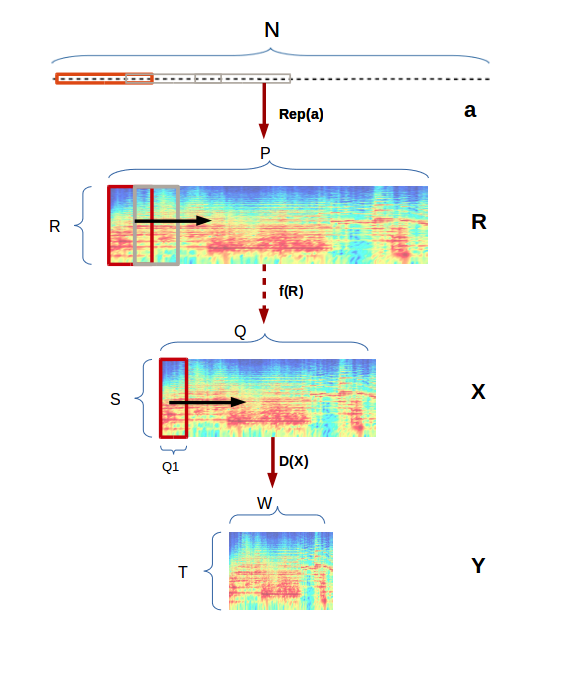
\includegraphics[width=0.7\textwidth]{dim_red}
\caption{Dimensionality Reduction Pipeline}
 \label{fig:Dimensionality Reduction}
 \end{figure}
\FloatBarrier
\bigskip

\subsection{Domain engineering Vs Unsupervised learning Vs Supervised learning}
\textit{Reduction by Domain engineering :} When the operators performing reduction are computed using the domain specific properties of the data, then the resulting reduction is said to be \textit{engineered}. Coming up with such operators is usually time-consuming and requires expert knowledge.\\
\\
\textit{Reduction by Unsupervised learning :} When the operators performing reduction are computed by exploiting the representation \textit{structure} of the data, then the resulting reductions are said to be \textit{learned} from the data. When this learning problem \textit{does not} require any labelled data, then the reduction is said to be \textit{unsupervised}.\\
\\
\textit{Reduction by Supervised learning :} When the operators performing reduction computed by exploiting the information from labelled data, then the resulting reduction is said to be obtained by \textit{supervised learning} 

\subsection{Principal Component Analysis (PCA)}
\label{pca}

The representation $\textbf{X}$ is changed to a \textit{basis} that are functions of variance between the frequency components. This is done by computing the co-variance matrix $\bm{\Sigma}$ from the data and performing \textit{orthogonal decomposition} to compute it's basis. The co-ordinates of the resulting basis system are called \textit{principal components}. The key idea for reduction is to discard the information corresponding to \textit{low variance} basis. The computation of PCA reduction operator $\textbf{W}_{PCA}$ is elaborated below,  

\begin{enumerate}[label=(\alph*)]
\item Usually, large samples (say $S$ samples) of representations from the dataset ($ \textbf{S} = [\textbf{X}_{1}, \textbf{X}_{2}, ..., \textbf{X}_{S}])$ are used to compute the co-variance matrix. The columns of $\textbf{S}$ are centred by their mean and the covariance matrix is computed as,
\[
   \bm{\Sigma} = \textbf{E}[(\textbf{S} - \textbf{E}[\textbf{S}])(\textbf{S} - \textbf{E}[\textbf{S}])^{T}] = \frac{1}{\displaystyle\sum_{s}{P_{s}}}\textbf{\^S}\textbf{\^S}^{T} \quad \in \mathbb{S}^{R \times R}
\]
The covariance matrix $\bm{\Sigma}$ is symmetric positive definite and hence belongs to space of symmetric operators $\mathbb{S}$.
\item The eigen values and eigen vectors of $\bm{\Sigma}$ are computed. At this point, we use the Orthogonal Eigenvector Decomposition Theorem and infer that eigen vectors of symmetric matrix ($\bm{\Sigma}$) form an orthogonal basis in $\mathbb{R}^{R}$. 
\[
\bm{\Sigma} = \textbf{V}\bm{\Lambda}\textbf{V}^{T} \qquad \textbf{V} \in \mathbb{O}^{R \times R}, \quad \bm{\Lambda} \in \mathbb{D}^{R \times R}
\]
The columns of matrix $\textbf{V}$ form the basis. Since the columns are orthogonal to each other, $\textbf{V}$ belongs to a space of orthogonal operators $\mathbb{O}$. $\bm{\Lambda}$ is a diagonal matrix of eigen values.

\item The eigen values represent the magnitude of variance for each frequency dimension.  Hence, eigenvectors corresponding to large eigen values gives the coordinates corresponding to greater variance. So eigen vectors corresponding to top $T$ eigen values are retained, while ignoring coordinates of lower variance. The resulting change of coordinates matrix is then $\textbf{\^V} \in \mathbb{O}^{R \times T}$
   
\item Since $\textbf{\^V}$ is orthogonal, $\textbf{\^{V}}^{-1} = \textbf{\^{V}}^{T}$, and the resulting reduction for \textit{each sample} can computed as $\textbf{Y} = \textbf{\^{V}}^{T}\textbf{X}$, where $\textbf{X} \in \mathbb{R}^{R \times P}$, $\textbf{Y} \in \mathbb{R}^{T \times P}$ and $T < R$. Thus the reduction operator is
\[
\textbf{W}_{PCA} = \textbf{\^V}^{T}
\]

\end{enumerate}   

\begin{algorithm}
  \caption{$\textbf{W}_{PCA}$ = PCA($\textbf{X}_{1}, \textbf{X}_{2},..,\textbf{X}_{S}$)}\label{alg:pca}
  \begin{algorithmic}[1]
    \Statex \textbf{Input :} $\textbf{S} = [\textbf{X}_{1},..\textbf{X}_{S}] \qquad \textbf{X}_{s} \in \mathbb{R}^{R \times P_{s}}, \textbf{S} \in \mathbb{R}^{R \times Q},\qquad  Q = \displaystyle\sum_{s}{P_{s}}$
    \Statex \textbf{Output :} $\textbf{W}_{PCA} \in \mathbb{R}^{T \times R}$
      \State $\bm{\Sigma} = \frac{1}{Q}\textbf{S}\textbf{S}^{T}$ \Comment{$\bm{\Sigma} \in \mathbb{S}^{R \times R}$}
      \State $\textbf{V}^{T} \bm{\Lambda} \textbf{V} = \bm{\Sigma}$ \Comment{$\bm{\Lambda} \in \mathbb{D}^{R \times R}$ , $\textbf{V} \in \mathbb{O}^{R \times R}$}
      \State $\textbf{V} \leftarrow \textbf{V}[:][:T]$ \Comment{$\textbf{V} \in \mathbb{O}^{R \times T}$}
      \State $\textbf{W}_{PCA} = \textbf{V}^{T}$
  \end{algorithmic}
\end{algorithm}
\FloatBarrier

\noindent Since the operator $\textbf{W}_{PCA}$ is computed from the data without requiring labelling, this method falls under \textit{unsupervised learning}. The columns of representation are first centred before applying the PCA reduction operation. An illustration of PCA reduction function $D_{(PCA)}$ is shown below,

\begin{algorithm}
  \caption{$\textbf{Y}$ = $D_{(PCA)}$($\textbf{X}$)}\label{alg:dpca}
  \begin{algorithmic}[1]
    \Statex \textbf{Input :} $\textbf{X} \in \mathbb{R}^{R \times P}$
    \Statex \textbf{Output :} $\textbf{Y} \in \mathbb{R}^{T \times P}$
	\State $\textbf{\^X} = \textbf{X} - \textbf{E}[\textbf{X}]$
	\State $\textbf{Y} = \textbf{W}_{PCA}\textbf{\^X}$
  \end{algorithmic}
\end{algorithm}
\FloatBarrier

\noindent Sometimes, to make the resulting reduction $\textbf{Y}$ uncorrelated (the resulting transformation should have identity co-variance matrix), the corresponding dimensions are divided by their eigen values. This is because eigen values are proportional to the magnitude of variance in each frequency direction. This operation is known as \textbf{PCA Whitening} and the reduction operator is,
\[
\textbf{W}_{PCAW} = \bm{\Lambda}^{-1}\textbf{\^V}^{T}
\]    
The reduction function $D_{(PCAW)}$ is same as algorithm \ref{alg:dpca}, except that the operator $\textbf{W}_{PCAW}$ is used instead of $\textbf{W}_{PCA}$
\bigskip

\subsection{Mel-frequency cepstrum coefficients (MFCC)}
\label{mfcc}
It has been studied that the basis functions resulting from co-variance matrix of log-mel spectrogram representation are similar to cosine transform on log-mel spectrogram\cite{mfcc_pca}. Therefore, instead of explicitly computing the basis functions from the data, one can simple use cosine basis. The co-ordinates of corresponding basis system are known as \textit{Mel-Frequency Cepstrum Coefficients}. The co-ordinates of high frequency cosine functions are discarded because they correspond to low-variance information. 
\bigskip

\noindent This reduction is engineered only for log mel spectrogram representation. $\textbf{W}_{MFCC}$ is the reduction operator.

\begin{algorithm}
  \caption{$\textbf{Y}$ = $MFCC$($\textbf{a}$) }\label{MFCC}
  \begin{algorithmic}[1]
    \Statex \textbf{Input :} $\textbf{a} \in \mathbb{R}^{N}$
    \Statex \textbf{Output :} $\textbf{Y} \in \mathbb{R}^{T \times P}$
    \State $\textbf{X} = R_{(MEL)} \big( \textbf{a} \big) $ \Comment{$\textbf{X} \in \mathbb{R}^{R \times P} $} 
    \State $\textbf{X} \leftarrow ln(\textbf{X})$
    \For{$ \omega \in \{1,..,T\}$}
    \State $\textbf{W}_{MFCC}[ \omega ] \leftarrow \textbf{cos}( \omega \textbf{t})$  \Comment{$\textbf{W}_{MFCC} \in \mathbb{R}^{R \times T}, \textbf{t} \in \mathbb{R}^{R}$}
    \EndFor
    \State $\textbf{Y} \leftarrow \textbf{W}_{MFCC}\textbf{X}$
  \end{algorithmic}
\end{algorithm}
 

\subsection{Convolution neural network}
\label{stacked}
Transformation of input $\textbf{a}$ by shifted contractions of an operator $\textbf{w}$ is termed as \textit{discrete convolution} and can be mathematically represented as one dimensional convolution operation, 
\[
	\textbf{y} = \textbf{a} \star \textbf{w}^{(s)}
\]   
The operator $\textbf{w}$ is known as a \textit{filter function} and the length of shift $s$ is known as \textit{stride}. Usually $\textbf{a}$ is convolved with multiple filter functions. For $K$ \textit{filters},
\[
	\textbf{Y}[k] = \textbf{a} \star {\textbf{w}_{k}}^{(s)} = \textbf{a} \star \textbf{W}^{(s)} \qquad k \in {0,1..K-1}
\] 
The index based notations for this operation are shown in appendix \ref{1dconv}. If the filters $\textbf{w}_{k}$ are \textit{defined}, then computation of $\textbf{Y}$ is straight forward. All the operations explained in the previous section are forward convolutions with defined filters,
\begin{itemize}
\setlength\itemsep{0em}

\item \textbf{STFT} in equation \ref{eq:stft}, where the filter functions are complex negative exponentials.
\item Transformation to \textbf{Mel} frequency scale in equation \ref{eq:mel}, where a set of mel-frequency centred filters are used.
\item \textbf{Principal components} and \textbf{MFCC} can be realized as a convolution of the input with transformation matrix $\textbf{V}^{T}$ defined in section \ref{pca} (Recall that matrix multiplication can be represented as a convolution of stride equal to column length. An illustration was shown in section \ref{mel})  

\end{itemize}
However, it is not clear if such defined filters really encodes the information in $\textbf{Y}$ relevant for certain context-based classification task. But, when a set of task-specific observations are available, it is possible to solve for the filters $\textbf{w}_{k}$, so that the resulting transformation $\textbf{Y}$ is optimal for the considered task. This is done using iterative optimization techniques, starting by random initializing of $\textbf{w}_{k}$ and updating it's values after every iteration. Computational models that solves by \textbf{first-order gradient descent} methods (a class of optimization techniques) are represented as first order \textbf{artificial neural networks}. The filters $\textbf{w}_{k}$ which we are attempting to solve are also termed as \textit{parameters} or \textit{weights} of the network. The iterative steps involving finding these \textit{weights} is termed as \textit{training} the neural network (Details of training neural network are explained in section \ref{training}). Since the transformation operation by the \textit{filters} are represented as convolution over the input, the neural network is termed as \textbf{convolution neural network}.   

\subsubsection{Approximating MFCC with CNN}
\textit{Supervised} feature learning has an advantage over \textit{unsupervised} feature learning when we wish to find filters $\textbf{w}_{k}$ optimal for context based classification tasks. Feature learning with CNN fall under \textit{supervised} feature learning category.
To show that CNN can do atleast as good as MFCCs, an illustration is discussed by approximating MFCC with CNN. Setting up a CNN architecture requires defining the \textit{hyper parameters} like number of filters, filter dimensions and stride of the filter. The domain knowledge of MFCC computation is used to set these hyper parameters.
\bigskip  

\noindent To compute MFCC features, the input signal $\textbf{a}$ is convolved with complex negative exponentials ($\textbf{W}_{STFT}$). After element-wise squaring operation, the resulting transformation is convolved with mel-filters ($\textbf{W}_{MEL}$). Logarithm of the resulting transformation is then convolved with cosine filters ($\textbf{W}_{MFCC}$). The motivation and description of these so called \textit{engineered} filters were described in section \ref{time} and \ref{dimension}. 

\begin{algorithm}
  \caption{$\textbf{Y}$ = MFCC($\textbf{a}$) }\label{MFCC_engineer}
  \begin{algorithmic}[1]
    \Statex \textbf{Input :} $\textbf{a} \in \mathbb{R}^{N}$
    \Statex \textbf{Output :} $\textbf{Y} \in \mathbb{R}^{T \times Q}$ 
    \State $\textbf{C} = \textbf{a} \star {\textbf{W}_{STFT}}^{(s)}$ \Comment{$ \textbf{W}_{STFT} \in \mathbb{R}^{M \times F}, \textbf{C} \in \mathbb{C}^{M \times Q}$}
    \State $\textbf{C} \leftarrow \textbf{C} \odot \textbf{C}$ 
    \State $\textbf{X} = \textbf{C} \star {\textbf{W}_{MEL}}^{(M)}$ \Comment{$ \textbf{W}_{MEL} \in \mathbb{R}^{R \times M}, \textbf{X} \in \mathbb{R}^{R \times Q}$}
    \State $\textbf{X} \leftarrow ln(\textbf{X})$
    \State $\textbf{Y} = \textbf{X} \star {\textbf{W}_{MFCC}}^{(R)}$ \Comment{$\textbf{W}_{MFCC} \in \mathbb{R}^{T \times R}$}
  \end{algorithmic}
\end{algorithm}
\FloatBarrier
\noindent An equivalent of MFCC computation can be realized with three layers of convolution by replacing the engineered filters by learnable filters and setting the following hyper parameters :
\begin{itemize}
\setlength\itemsep{0em}
\item $\textbf{W}_{L1}$ : $M$ filters (representing discrete frequencies) of size $F$ (STFT window size) and stride $s$ (STFT hop length)
\item $\textbf{W}_{L2}$ : $R$ filters (for mel-frequencies) of size $M$ and stride $M$.
\item $\textbf{W}_{L3}$ : $T$ filters (for mel coefficients) of size $R$ and stride $R$.   
\end{itemize}
The non-linearity in between each layer is needed. Otherwise, the filters accross layers can be combined into a representation for single layer. Setting $\bm{\Phi}_{1}$ as element-wise squaring operation and $\bm{\Phi}_{2}$ as logarithm should result in a CNN architecture that \textit{may} realize MFCCs. That is, the solution will converge to the defined filters ($\textbf{W}_{STFT}, \textbf{W}_{MEL}, \textbf{W}_{MFCC}$) if they are optimal for the task considered. Otherwise, one could expect either richer representation or sub-optimal representation because of local convergence.  
\begin{algorithm}
  \caption{$\textbf{Y}$ = CNN($\textbf{a}$) }\label{MFCC_learn}
  \begin{algorithmic}[1]
    \Statex \textbf{Input :} $\textbf{a} \in \mathbb{R}^{N}$
    \Statex \textbf{Output :} $\textbf{Y} \in \mathbb{R}^{T \times Q}$ 
    \State $\textbf{C} = \bm{\Phi}_{1} (\textbf{a} \star {\textbf{W}_{L1}}^{(s)})$ \Comment{$ \textbf{W}_{L1} \in \mathbb{R}^{M \times F}, \textbf{C} \in \mathbb{C}^{M \times Q}$}
    \State $\textbf{X} = \bm{\Phi}_{2} (\textbf{C} \star {\textbf{W}_{L2}}^{(M)})$ \Comment{$ \textbf{W}_{L2} \in \mathbb{R}^{R \times M}, \textbf{X} \in \mathbb{R}^{R \times Q}$}
    \State $\textbf{Y} = \bm{\Phi}_{3} (\textbf{X} \star {\textbf{W}_{L3}}^{(R)})$ \Comment{$\textbf{W}_{L3} \in \mathbb{R}^{T \times R}$}
  \end{algorithmic}
\end{algorithm}
\FloatBarrier
\noindent It is possible to with-hold the engineered filters at earlier levels and just introduce learning at later stages. For instance, it is sometimes optimal to compute the STFT and mel-filters and just perform convolutions over the mel-spectrogram\cite{EndToEnd}\cite{choi_cnn}. Sometimes it is also useful to generalize the convolution as a 2 dimensional operation\cite{MusicMotive}.(see Chapter 3, Sec. \ref{convolution}). 2D convolution operation is shown in appendix \ref{2dconv}. 

\subsubsection{CNN as a general purpose feature extractor}  
\label{general}
In music information retrieval, several task-specific features have been engineered. The MFCC features along with it's derivatives (the derivative is useful to encode the temporal evolution) are often used for genre and mood recognition tasks. Instead of convolving with mel-filters on STFT representation, one might opt for filters that would result in chroma-gram (combines frequencies by exploiting the periodicity of pitches) or tempo-gram (encodes change of frequencies over time). Features derived from chroma-gram find application for automatic mixing, chord recognition tasks. Features derived from tempo-gram find applications for tasks like on-set detection, tempo-estimation etc.. But more often, combination of features are used to boost classifier performance. For all these features that can be realized in terms of hierarchy of convolution operations, it is possible to find mathematical equivalence in convolution neural network.     

\begin{figure}[h] 
\centering
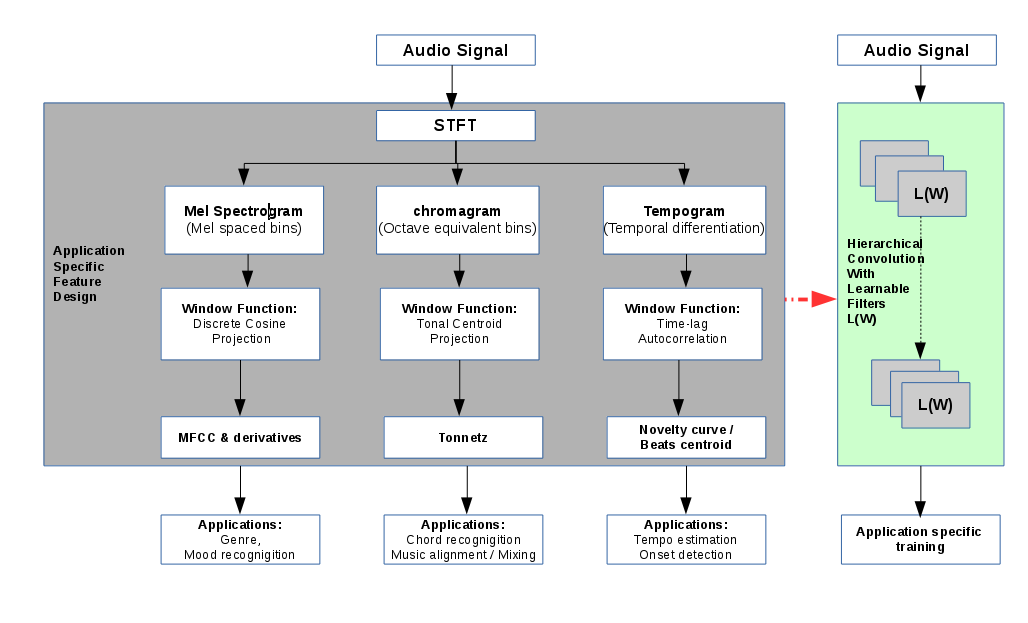
\includegraphics[width=0.95\textwidth]{dnn_motivation}
\caption{General purpose feature extractor}
 \label{fig:deep learning}
 \end{figure}
\FloatBarrier
\bigskip

\section{Temporal Approximation}
\label{temporal}
The size of resulting features computed through reduction operations discussed in the previous section depends on length of the audio. But classifiers like \textit{support vector machines} and \textit{multi layer perceptron} requires features of fixed size to compute the parameters while training. Therefore, frame-wise features over time are approximated to a fixed size feature representation. Temporal approximation $T$ of the reduced representation $\textbf{Y}$ is  
\[
\textbf{f} = T(\textbf{Y}) \qquad \textbf{f} \in \mathbb{R}^{Z}, \textbf{Y} \in \mathbb{R}^{T \times W}
\]
$W$ depends on length of the audio. $\textbf{f}$ is usually the final fixed size feature that is given as input to the classifier.  
\bigskip

\noindent The transformation by approximation function $T$ is done by using one of the methods,
\begin{itemize}
\setlength\itemsep{0em}
\item \textit{unsupervised} methods involving \textit{clustering techniques} (Bag Of Frames, Gaussian mixture models)
\item \textit{supervised} methods with \textit{recurrent neural network}. 
\end{itemize} 
 
\subsection{Bag Of Frames}
\label{clustering}
In Bag of Frames(BoF) model\cite{BoF}, the \textit{frequency} of each reduced frame is used as a feature for training a classifier. To reduce to a fixed size representation (of size $Z$), $Z$ cluster centres are computed from the data. Each frame-wise feature is assigned to it's nearest cluster. The number of assignments to each cluster now becomes the feature $\textbf{f}$. 
\begin{algorithm}
  \caption{$\textbf{f}$ = BagOfFrames($\textbf{Y}$) }\label{bof}
  \begin{algorithmic}[1]
    \Statex \textbf{Input :} $\textbf{Y} \in \mathbb{R}^{T \times W}$
    \Statex \textbf{Output :} $\textbf{f} \in \mathbb{R}^{Z}$
    \State $\textbf{f} = 0$
    \For{$ i \in \{0,1,..,W-1\}$}
    \State $j = \argmin\limits_{j} \norm{\textbf{Y}[:,i] - \bm{\mu}_{j}}^{2}$ \Comment{$\bm{\mu}_{j} \in \mathbb{R}^{T}, j \in \{0,1..Z-1\}$}
    \State $\textbf{f}[j] \leftarrow \textbf{f}[j] + 1$
    \EndFor
  \end{algorithmic}
\end{algorithm}
\FloatBarrier
\noindent The cluster centres are computed by clustering algorithms likes gaussian mixture models or K-Means clustering. Computation of $\bm{\mu}_{j}$ by K-Means is illustrated in algorithm \ref{alg:kmeans}. The cluster centres are computed for the entire dataset. Each of the $N$ sample track could have $W$ frame-wise features. To compute these centres, $\bm{\mu}_{j}$ are first randomly initialized. Then each frame level feature is assigned to the nearest centre. After the assignment of all frame features, the cluster centres $\bm{\mu}_{j}$ are re-computed. The frame features are then re-assigned to these new centres. This re-assignment and re-computation of $\bm{\mu}_{j}$ is iterated until convergence.  
\begin{algorithm}
  \caption{K-MEANS($\textbf{Y}_{0}, \textbf{Y}_{2},..., \textbf{Y}_{N-1}$) }\label{alg:kmeans}
  \begin{algorithmic}[1]
    \Statex \textbf{Input :} $\textbf{Y}_{n} \in \mathbb{R}^{T \times W}, n \in \{0,1,...,N-1\}$
    \Statex \textbf{Output :} $\bm{\mu}_{j} \in \mathbb{R}^{T}, j \in \{0,1,..,Z-1\}$
    \State Randomly initialize $\bm{\mu}_{j}$
    \While{$\bm{\mu}_{j}$ have not converged}
    \For{$n \in \{0,1,..,N-1$}
      \For{$ i \in \{0,1,..,W-1\}$}
         \State $j = \argmin\limits_{j} \norm{\textbf{Y}_{n}[:,i] - \bm{\mu}_{j}}^{2}$
          \State Assign $\textbf{Y}_{n}[:,i]$ to cluster $j$
      \EndFor
    \EndFor
   \State Recompute cluster means $\bm{\mu}_{j}$
   \EndWhile
  \end{algorithmic}
\end{algorithm}
\FloatBarrier

\subsection{Recurrent Neural Networks}
\label{rnn}
The idea behind RNN is to learn a feature representation by sequentially combining the input into an internal state $\textbf{h}$. The resulting feature ($\textbf{f}$) is a projection from this internal state.
\[ 
\textbf{f} = \textbf{W}\textbf{h}_{W} \qquad \textbf{W} \in \mathbb{R}^{Z \times K}, \textbf{h}_{W} \in \mathbb{R}^{K}
\]
\[
\textbf{h}_{W} = \bm{\Theta}(\textbf{Y}[:,W], \textbf{h}_{W-1}) \qquad \textbf{Y} \in \mathbb{R}^{T \times W}
\]
$\textbf{h}_{W}$ is the internal state after combining $W$ columns of $\textbf{Y}$. $\bm{\Theta}$ is the internal state function which sequentially combines the input. The operator $\textbf{W}$ and other operators resulting from the function $\bm{\Theta}$ are solved for optimality using a labelled dataset. These operators can be computed by training an RNN (see Section \ref{training}). The function $\bm{\Theta}$ should sufficiently hold the information from beginning to end of the sequence. RNNs face challenge in remembering the information in the earlier part of the sequence. Because of this, different flavours of RNN have been developed to hold the sequence information longer and to battle the vanishing gradient problem while training neural network (see Section \ref{training}). Depending on how $\bm{\Theta}$ is defined, at least two RNN architectures are popular in the literature: Long-Short Term Memory (LSTM) RNN and Gated Recurrent Unit(GRU) RNN. In this thesis, only LSTMs\cite{LSTM} are considered.   

\subsubsection{Long-Short Term Memory RNN}
The LSTM internal state is contained by three gates that control the information flow. This is done by multiplying the output of each sequence $\textbf{o}_{w}$ with the corresponding cell state function $\textbf{c}_{w}$.
\[
\textbf{h}_{w} = \textbf{o}_{w} \odot \sigma_{h}(\textbf{c}_{w}) \qquad w \in \{1,2,...,W\}
\] 
$\sigma_{h}$ is hyperbolic tangent function which projects the values between -1 and 1. The output gate $\textbf{o}_{w}$ combines the $w^{th}$ vector in sequence with the previous internal state ($\textbf{h}_{w-1}$) and projects the result between 0 and 1 with sigmoid activation ($\sigma$). This indicates the contribution of current sequence $w$ to the cell state. 
\[
\textbf{o}_{w} = \sigma(\textbf{W}_{o}\textbf{Y}[:,w] + \textbf{U}_{o}\textbf{h}_{w-1})
\]
The cell state $\textbf{c}_{w}$ acts as a conveyor belt where the information can either flow unchanged or get modified with update ($\textbf{i}_{w}$) and forget functions ($\textbf{g}_{w}$).
\[
\textbf{c}_{w} = \textbf{g}_{w} \odot \textbf{c}_{w-1} + \textbf{i}_{w} \odot \sigma_{h}(\textbf{W}_{c}\textbf{Y}[:,w] + \textbf{U}_{c}\textbf{h}_{w-1})
\] 
The operators of forget gate $\textbf{W}_{g}$ and $\textbf{U}_{g}$ control the deletion of information from the\textit{ previous} sequence. The output of $g_{w}$ is between 0 (delete the information) and 1 (keep the information). 
\[
\textbf{g}_{w} = \sigma(\textbf{W}_{g}\textbf{Y}[:,w] + \textbf{U}_{g}\textbf{h}_{w-1})
\] 
The operators of update gate $\textbf{W}_{i}$ and $\textbf{U}_{i}$ control the addition of information from the \textit{current} sequence. The output of $i_{w}$ is also between 0 and 1.
\[
\textbf{i}_{w} = \sigma(\textbf{W}_{i}\textbf{Y}[:,w] + \textbf{U}_{i}\textbf{h}_{w-1})
\] 
The operators $\textbf{W}_{o}, \textbf{U}_{o}, \textbf{W}_{i}, \textbf{U}_{i}, \textbf{W}_{g}, \textbf{U}_{g}, \textbf{W}_{c}$ and $ \textbf{U}_{c}$ are solved by training the RNN.
\bigskip

\noindent To get a fixed size temporal approximation, the RNN should project all the input sequence to a single output. This architecture of RNN is called \textit{Sequence to One} RNN. 
\begin{algorithm}
  \caption{$\textbf{f}$ = $Seq2One\_LSTM$($\textbf{Y}$) }\label{alg:s2olstm}
  \begin{algorithmic}[1]
    \Statex \textbf{Input :} $\textbf{Y} \in \mathbb{R}^{T \times W}$
    \Statex \textbf{Output :} $\textbf{f} \in \mathbb{R}^{Z}$
    \State Initialize $\textbf{h}_{0}$
    \For{$ w \in \{1,2,..,W\}$}
    \State  $\textbf{h}_{w} \leftarrow \bm{\Theta}_{LSTM}(\textbf{Y}[:,w],\textbf{h}_{w-1})$
    \EndFor
    \State $\textbf{f} = \textbf{W}\textbf{h}_{W}$
  \end{algorithmic}
\end{algorithm}
\FloatBarrier

\noindent Often times, multiple layers of RNN are used. An illustration of  two layer LSTM with a \textit{sequence to sequence} LSTM in between is shown in algorithm \ref{alg:2lstm}. The input sequence transformed in to a hidden sequence, which is then projected to a single output by the second layer. The functions in between ($\Phi_{1}, \Phi_{2}$) represents the transition operation between the layers. Several non-linear activations and transition operations have been developed to address the problems while training deep neural network (see Sec. \ref{training}). 
  
\begin{minipage}[t]{7.5cm}
  \vspace{0pt}  
\begin{algorithm}[H]
  \caption{$\textbf{f}$ = $LSTM2(\textbf{Y})$}\label{alg:2lstm}
  \begin{algorithmic}[1]
    \Statex \textbf{Input :} $\textbf{Y} \in \mathbb{R}^{T \times W}$
    \Statex \textbf{Output :} $\textbf{f} \in \mathbb{R}^{Z}$
    \Statex
    \Statex
    \Statex
    \State $\textbf{F}_{1} = \Phi_{1}(Seq2Seq\_LSTM(\textbf{Y}))$
    \State $\textbf{f} = \Phi_{2}(Seq2One\_LSTM(\textbf{F}_{1})$
  \end{algorithmic}
\end{algorithm}
\end{minipage}%
\begin{minipage}[t]{7.5cm}
  \vspace{0pt}
\begin{algorithm}[H]
  \caption{$\textbf{F}$ = $Seq2Seq\_LSTM$($\textbf{Y}$) }\label{alg:s2slstm}
  \begin{algorithmic}[1]
    \Statex \textbf{Input :} $\textbf{Y} \in \mathbb{R}^{T \times W}$
    \Statex \textbf{Output :} $\textbf{F} \in \mathbb{R}^{Z \times W}$
    \State Initialize $\textbf{h}_{0}$
    \For{$ w \in \{1,2,..,W\}$}
    \State  $\textbf{h}_{w} \leftarrow \bm{\Theta}_{LSTM}(\textbf{Y}[:,w],\textbf{h}_{w-1})$
    \State $\textbf{F}[:,w] = \textbf{W}\textbf{h}_{W}$
    \EndFor
  \end{algorithmic}
\end{algorithm}
\end{minipage}
\FloatBarrier

\section{Multi-label Classifier}
\label{classifier}
The classifier takes the feature $\textbf{f}$ as input and performs the classification task. A \textit{discriminative} \footnote{The classification model can either be \textit{generative} (approximates class distribution) or \textit{discriminative} (approximates class boundaries). For a binary classifier, the classes are either 0 or 1} binary classifier can be formalised as, 
\[
\ell_{i} = b(\zeta_{i}) =
\begin{cases}
1, & \text{if  } \zeta_{i} > \epsilon \\
0, & \text{otherwise}
\end{cases}
\qquad i \in \{1,2,..,L\}, \ell_{i} \in \{0,1\}, \textbf{f} \in \mathbb{R}^{Z}
\]
where $b$ is a binary classifier, given the feature vector $\textbf{f}$. The output of a binary classifier $\ell_{i}$ is either 0 or 1. There are $L$ binary classifier outputs for $L$ labels. $\zeta_{i}$ is the $i^{th}$ output of the classification function $C$ and the classifier output $\ell_{i}$ is 1 if $\zeta_{i}$ is greater than certain threshold $\epsilon$ 
\[
\bm{\zeta} = C(\textbf{f}) \qquad \bm{\zeta} \in \mathbb{R}^{L}
\]
The final prediction ($\textbf{pred}$) is an index set of all classifier outputs that is equal to 1 
\[
\textbf{pred} = \{\ell_{i} | \ell_{i} = 1 \}
\]
The following equivalent notation will be used in algorithms of upcoming chapters 
\[
\textbf{pred}_{(\epsilon)} = \{ b(\zeta_{i}) | b(\zeta_{i}) = 1 \} \qquad i \in \{1,2,..,L\}
\]
The classification function $C$ projects the feature $\textbf{f}$ to the vector $\bm{\zeta}$ in the label space. Depending on how this function is defined, there are several discriminative classifiers like \textit{multi-layer perceptrons}, \textit{support vector machines}, \textit{random-forest}. In this thesis, only \textit{multi-layer perceptron} is considered.


\subsection{Two-layer perceptron}
A two layer perceptron first projects the features $\textbf{f}$ to a hidden layer $\textbf{h}$ and some element-wise non-linear operation $\Phi$ is applied.
\[
\textbf{h} = \Phi(\textbf{W}_{L1}\textbf{f}) \qquad \textbf{h} \in \mathbb{R}^{L1}, \textbf{W}_{L1} \in \mathbb{R}^{L1 \times Z}
\]
Without the non-linear operation $\Phi$, the operators $\textbf{W}_{L1}$ and $\textbf{W}$ can multiply out to generalize a single layer perceptron. The motivation for using a two layer perceptron is because single layer perceptron can approximate only linear class boundries. But \textit{universal approximation theorem}\cite{upt} states that a single hidden layer with some non-linear activation function can approximate any function. The choice of $\Phi$ will be explained in section \ref{training}. The second operator $\textbf{W}$ performs the projection from hidden vector $\textbf{h}$  
\[
\bm{\zeta} = \sigma (\textbf{W}\textbf{h}) \qquad \bm{\zeta} \in \mathbb{R}^{L}, \textbf{W} \in \mathbb{R}^{L \times L1}
\]
where $\sigma$ is a sigmoid function, which projects the output of second layer between 0 and 1. 
\begin{equation}
\label{sigmoid}
\sigma (x) = \frac{1}{1 + e^{-x}}
\end{equation}
Thus $0 \leq \zeta_{i} \leq 1$ and threshold $\epsilon$ can be set in-between 0 and 1 and eventually the final prediction $\textbf{pred}$ can be computed. 

\section{Training}
\label{training}
The iterative steps involving the computation of the operators that is optimal for transformations for our context-based classification task is called \textit{training}. When we train only the operators of classifying function $C$ (that is, $\textbf{W}$ and $\textbf{W}_{L1}$), the classification performance will only be as good as the information encoded in the feature $\textbf{f}$. Let us assume that the features $\textbf{f}$ obtained as a result of transformations $R$, $D$, and $T$ is optimal for the task at hand. Hence, only the classifier $C$ is trained. The abstract prediction model is shown in algorithm \ref{abstraction}.
\begin{algorithm}
  \caption{$\textbf{pred}$ = $Model$($\textbf{a}$) }\label{abstraction}
  \begin{algorithmic}[1]
    \Statex \textbf{Input :} $\textbf{a} \in \mathbb{R}^{N}$
    \Statex \textbf{Output :} $\textbf{pred}$ \Comment{indices of predicted labels}
    \State $\textbf{X} = R(\textbf{a})$ \Comment{$\textbf{X} \in \mathbb{R}^{R \times P}$}
    \State $\textbf{Y} = D(\textbf{X})$ \Comment{$\textbf{Y} \in \mathbb{R}^{T \times W}$}
    \State $\textbf{f} = T(\textbf{Y})$ \Comment{$\textbf{f} \in \mathbb{R}^{Z}$}
    \State $\bm{\zeta} = C(\textbf{f} \quad |\textbf{W},\textbf{W}_{L1})$ \Comment{$\bm{\zeta} \in \mathbb{R}^{L}$}
    \State $\textbf{pred} = \{ b(\zeta_{i}) | b(\zeta_{i}) = 1 \}$ \Comment{$ i \in \{1,2,..,L\}, b( \zeta_{i}) \in \{0,1\}$}
  \end{algorithmic}
\end{algorithm}
\FloatBarrier
\noindent Considering a two layer perceptron for classification, $\bm{\zeta}$ is computed as,
\begin{equation}
\label{eq:mlp}
\bm{\zeta} = \sigma ( \textbf{W} \Phi (\textbf{W}_{L1}\textbf{f}))
\end{equation}
\noindent Computing $\textbf{W}$ and $\textbf{W}_{L1}$ is an inverse problem. That is, we need a target $\textbf{t}$ that approximates $\bm{\zeta}$ for true classifications from a set of observations. To do this, recall that $\bm{\zeta}$ is a $L$ dimensional vector and $L$ is the number of labels in consideration. $\zeta_{i}$ is the classifier output for $i^{th}$ label and $i \in \{1,2,..,L\}$. With sigmoid ($\sigma$) projection we know that $0 \leq \zeta_{i} \leq 1$. If we assume $t_{i}$ equal to 1 for true classifications and 0 for the rest, then the transformation operators ($\textbf{W}$ and $\textbf{W}_{L1}$) can be solved such that the classifier output $\zeta_{i}$ is close to 1 for true classifications.

\subsection{First-order gradient descent}
Solving for the operators by \textit{first-order gradient descent} involves the following steps : 
\begin{enumerate}
\setlength\itemsep{0em}
\item Initialize $\textbf{W}, \textbf{W}_{L1}$
\item Run the model for a sample and compute loss $E$ = $loss(\bm{\zeta}, \textbf{t})$
\item Compute the gradient of loss with respect to the operators ($ \frac{\partial E}{\partial \textbf{W}}, \frac{\partial E}{\partial \textbf{W}_{L1}}$)
\item Update $\textbf{W}$ and $\textbf{W}_{L1}$
\item Recompute loss, gradients and update the parameters until convergence.
\end{enumerate}

\subsubsection{Loss function}
To train a classifier, a loss function (or error function) have to be defined. The \textit{least square} error function is sensitive to outliers in the training data. Hence \textit{cross-entropy}\cite{ml} loss function is considered. Error function defined as the negative log-likelihood is the \textit{cross-entropy} error function. \textit{Likelihood} that the parameters ($\textbf{W}, \textbf{W}_{L1}$) approximate a set of targets for label $i$ for $N$ training samples $({t_{i}}^{1}, {t_{i}}^{2},...,{t_{i}}^{N})$ is
\[
\mathcal{L} (\textbf{W}, \textbf{W}_{L1} | {t_{i}}^{1}, {t_{i}}^{2},...,{t_{i}}^{N} ) =  \displaystyle\prod_{n=1}^{N} {\zeta_{i(n)}}^{{t_{i}}^{(n)}}{(1-\zeta_{i(n)})}^{1 - {t_{i}}^{(n)}} \qquad t_{i} \in \{0,1\}
\]
where the \textit{likelihood} is 1, as the classifier output $\zeta_{i}$ approaches the target $t_{i}$. The log-likelihood is taken to get rid of the multiplication that would cause numerical problems over large $N$. The negative of the log-likelihood is taken to pose the optimization as a \textit{minimization} problem. Therefore, minimizing the \textit{cross-entropy} loss for label $i$ is equivalent to minimizing the \textit{negative log likelihood}
\[
\text{Minimize } E_{i}  = -ln(\mathcal{L}) = - \displaystyle\sum_{n=1}^{N} \{ {t_{i}}^{(n)} ln \zeta_{i(n)} + (1-{t_{i}}^{(n)}) ln (1-\zeta_{i(n)}) \}
\]
For $L$ labels, the total loss is minimized,
\[
\text{Minimize } \displaystyle\sum_{i=1}^{L}E_{i} 
\]
Moreover, with gradient descent optimization, the loss is minimized for a batch of samples ($B$) for every iteration. $B$ is called the \textit{batch-size}. Thus, loss for every iteration would be,
\[
{E_{i}}^{(B)} = - \displaystyle\sum_{i=1}^{L}\displaystyle\sum_{n=1}^{B} \{ {t_{i}}^{(n)} ln \zeta_{i(n)} + (1-{t_{i}}^{(n)}) ln (1-\zeta_{i(n)}) \}
\]

\subsubsection{Computing gradients}
After every iteration, the gradient of the total loss ($E$) with respect to the parameters ($\textbf{W}, \textbf{W}_{L1}$) have to computed. This gradient will then be used to update the parameters for next iteration. The gradients are computed by applying the chain rule. An illustration for computing the gradients for the two layer perceptron is shown
\begin{equation}
\label{grad1}
\frac{\partial E}{\partial \textbf{W}} = \frac{\partial E}{\partial \bm{\zeta}}  \frac{\partial \bm{\zeta}}{\partial \sigma}  \frac{\partial \sigma}{\partial \textbf{W}}
\end{equation}
\begin{equation}
\label{grad2}
\frac{\partial E}{\partial \textbf{W}_{L1}} = \frac{\partial E}{\partial \bm{\zeta}}  \frac{\partial \bm{\zeta}}{\partial \sigma}  \frac{\partial \sigma}{\partial \Phi} \frac{\partial \Phi}{\partial \textbf{W}_{L1}}
\end{equation}
Efficient computation of the gradients is achieved with \textit{back-propagation} algorithm. To ease the computations, the non-linearities and loss functions are usually chosen in such a way that the variables required for gradient computation are known in the forward pass.

\subsubsection{Updating the parameters}
Standard stochastic gradient descent update for every iteration is,
\[
\textbf{W} = \textbf{W} - \eta \frac{\partial E}{\partial \textbf{W}}
\]
where $\eta$ is the learning rate. But choosing a proper learning rate is difficult because if $\eta$ is too small, convergence can be too slow, while $\eta$ that is too high can hinder convergence. Additionally, the same learning rate is applied to all parameters across the layers. Moreover, the neural networks lead to highly non convex optimization problem and to avoid getting trapped in a local optima is challenging. Therefore, several optimization algorithms specialized for neural network training emerged to deal with the aforementioned challenges. In this thesis, Adaptive Moment (ADAM) Estimation updates\cite{adam} will be used. ADAM uses the exponentially decaying average of past moments (first moment $m$ and second moment $v$) and squared gradients ($g$) to update the parameters. Update for iteration $t$ is,
\[
m_{t} = \beta_{1}m_{t-1} + (1- \beta_{1})g_{t}
\]
\[
v_{t} = \beta_{2}v_{t-1} + (1-\beta_{2}){g_{t}}^{2}
\]
As $m_{t}$ and $v_{t}$ are initialized as vectors of 0's, the authors of ADAM observe that they are biased towards zero, especially during the initial time steps, and especially when the decay rates are small (i.e. $\beta_{1}$ and $\beta_{2}$ are close to 1). They counteract these biases by computing bias-corrected first and second moment estimates\cite{adam_o}:
\[
{m}_{t} = \frac{m_{t}}{1-{\beta_{1}}^{t}}
\]
\[
{v}_{t} = \frac{v_{t}}{1-{\beta_{2}}^{t}}
\]
Thus, update of each parameter for the next iteration is,
\[
W_{t+1} = W_{t} - \frac{\eta}{\sqrt{v_{t}} + \epsilon}m_{t}
\]
The authors propose default hyper-parameter values of 0.9 for $\beta_{1}$, 0.999 for $\beta_{2}$, and ${10}^{-8}$ for $\epsilon$

\subsection{Deep learning}
As mentioned before, if we train only the operators of classifying function $C$, then the classification performance will only be as good as the information encoded in the feature $\textbf{f}$. But, if it is possible to solve for the transformation operators that compute the features $\textbf{f}$, then it is possible to obtain features optimal for the considered task. That is, if we push the supervision into the temporal approximator function $T$ with a \textit{sequence to one} LSTM, then the classifier performance is no longer limited by the encodings in the feature $\textbf{f}$. Because, now the operators of RNN can be solved for optimality in addition to the operators of 2 layer perceptron, and therefore $\textbf{f}$ can be optimal for the task. Now we have to update every iteration not just $\textbf{W}, \textbf{W}_{L1}$, but also $\textbf{W}_{o}, \textbf{U}_{o}, \textbf{W}_{i}, \textbf{U}_{i}, \textbf{W}_{g}, \textbf{U}_{g}, \textbf{W}_{c}$ and $ \textbf{U}_{c}$   

\begin{algorithm}
  \caption{$\textbf{pred}$ = $Model$($\textbf{a}$) }\label{abstraction2}
  \begin{algorithmic}[1]
    \Statex \textbf{Input :} $\textbf{a} \in \mathbb{R}^{N}$
    \Statex \textbf{Output :} $\textbf{pred}$ \Comment{indices of predicted labels}
    \State $\textbf{X} = R(\textbf{a})$ \Comment{$\textbf{X} \in \mathbb{R}^{R \times P}$}
    \State $\textbf{Y} = D(\textbf{X})$ \Comment{$\textbf{Y} \in \mathbb{R}^{T \times W}$}
    \State $\textbf{f} = Seq2One\_LSTM(\textbf{Y} \quad | \textbf{W}_{k}, \textbf{U}_{k})$ \Comment{$ k = \{ i_{r},o,g,c\}, \textbf{f} \in \mathbb{R}^{Z}$}
    \State $\bm{\zeta} = C(\textbf{f} \quad |\textbf{W},\textbf{W}_{L1})$ \Comment{$\bm{\zeta} \in \mathbb{R}^{L}$}
    \State $\textbf{pred} = \{ b(\zeta_{i}) | b(\zeta_{i}) = 1 \}$ \Comment{$ i \in \{1,2,..,L\}, b( \zeta_{i}) \in \{0,1\}$}
  \end{algorithmic}
\end{algorithm}
\FloatBarrier
\noindent However, the performance is still limited by the frame-wise features $\textbf{Y}$. But the supervision can be further pushed inside by using convolution neural networks and solving for it's operators ($\textbf{W}_{C1}, \textbf{W}_{C2}, \textbf{W}_{C3}$) in addition to the operators of RNN and perceptron.
\begin{algorithm}
  \caption{$\textbf{pred}$ = $Model$($\textbf{a}$) }\label{abstraction3}
  \begin{algorithmic}[1]
    \Statex \textbf{Input :} $\textbf{a} \in \mathbb{R}^{N}$
    \Statex \textbf{Output :} $\textbf{pred}$ \Comment{indices of predicted labels}
    \State $\textbf{X} = R(\textbf{a})$ \Comment{$\textbf{X} \in \mathbb{R}^{R \times P}$}
    \State $\textbf{Y} = CNN(\textbf{X} \quad | \textbf{W}_{C1}, \textbf{W}_{C2}, \textbf{W}_{C3})$ \Comment{$\textbf{Y} \in \mathbb{R}^{T \times W}$}
    \State $\textbf{f} = Seq2One\_LSTM(\textbf{Y} \quad | \textbf{W}_{k}, \textbf{U}_{k})$ \Comment{$ k = \{ i_{r},o,g,c\}, \textbf{f} \in \mathbb{R}^{Z}$}
    \State $\bm{\zeta} = C(\textbf{f} \quad |\textbf{W},\textbf{W}_{L1})$ \Comment{$\bm{\zeta} \in \mathbb{R}^{L}$}
    \State $\textbf{pred} = \{ b(\zeta_{i}) | b(\zeta_{i}) = 1 \}$ \Comment{$ i \in \{1,2,..,L\}, b( \zeta_{i}) \in \{0,1\}$}
  \end{algorithmic}
\end{algorithm}
\FloatBarrier
\noindent From the illustration in algorithm \ref{MFCC_learn}, it can be seen that the learning problem can pushed up to the point of even replacing the $STFT$ operators. That is, the model can be now trained to detect the pattern directly from the raw audio signal for our classification task. Since the training data is now able to affect the operators of feature computations, the context of learning problem is now called \textit{deep learning} 

\subsubsection{Issues}
\label{issues}
As exciting as it may sound, deep learning has two major issues,\\
\\
\textit{\textbf{Requires large training data} :}\\
\\
Looking at all the application domains where deep learning is successful (image /speech recognition), they are the ones where acquiring a lot of data is feasible. As the number of parameters to optimize increases, not only that more iterations are needed to converge, but there is also a risk that the solutions converge to learning the noise in data. This is called \textit{over-fitting}.\\
\\
\textit{Transfer-learning :} This is one way to address this issue for smaller datasets. \textit{Transfer learning} is possible only when an alternate large dataset for similar task (\textit{source task}) is available. It is  then possible to train with the smaller dataset by initializing the weights with the values converged in the source task. This is called \textit{fine-tuning} the model.\\
\\
\textit{Drop-out :} This is a regularizer that counter over fitting by randomly setting parameters to zero. This is called \textit{dropping} the connection. At each training iteration, the connections can be \textit{dropped out} with probability $p$. ($Drop_{(p)}$)\\  
\\
\textit{\textbf{Vanishing gradients} :}\\  
\\
As the number of layers in the neural network increases, the risk of gradients approaching zero in the earlier layers increases. This will increase the number of iterations required for convergence. As an illustration, looking at the gradient computation equations for the final layer in equation \ref{grad1} and the penultimate layer in equation \ref{grad2}, it can be seen that as we move deeper, the number of multiplications in the chain rule required for calculating the gradient increases. If one of those gradients in chain have a value close to zero, then the gradient with respect to the parameters will also be close to zero. Thus, the non-linearities $\Phi$ are chosen such that the gradient is boosted. The non-linearities - Rectified linear units ($ReLU$)\cite{relu} and Exponential linear units ($ELU$)\cite{elu} have been used in this thesis.  
\[
ReLU(x) = max(0,x)
\]     
\[
ELU(x) = 
\begin{cases}
x, & \text{if } x \geq 0 \\
a(e^{x}-1), & \text{otherwise}
\end{cases}
\]
where $a > 0$ is a hyper-parameter. 
\chapter{Literature Dynamics and Model Selection } % Main chapter title

\label{Chapter3} % For referencing the chapter elsewhere, use \ref{Chapter2} 

Using content-based music information for solving several music information retrieval tasks is not new, but a decade long research efforts have been put. Hunting for the right model for our task and to justify it to be superior to the rest requires thorough understanding of evolution of such techniques. In section 3.1, the dynamics of the literature that has lead to the use of deep learning techniques for MIR tasks have been discussed. In section 3.2, the inferences from state of art techniques have been used to short list models for the experiments.       


\section{Literature Review}
A number of surveys (e.g. [8, 22, 29]) amply document what is a decades-long research effort at the intersection of music, machine learning and signal processing. In a broader sense, all techniques have a two-stage architecture: first, features are extracted from music audio signals to transform them into a more meaningful representation. These features are then used as input to a classifier, which is trained to perform the task at hand. This dedicated analysis for music features emerged due to the fact that music signals possess specific acoustic and structural characteristics that distinguish them from spoken language or other non musical signals.
\bigskip

\noindent In a general sense, the goal of classification tasks in music informatics is to attach a semantic meaning to the content. The underlying issue is ultimately one of \textit{organization} and \textit{variance} of the features. 
\bigskip

\noindent \textit{\textbf{•Feature organization :}} The better organized a feature is to answer some question, the simpler it is to assign or infer semantic meaning. Thus a feature representation should explicitly reflects a desired semantic organization.

\noindent \textit{\textbf{•Feature variance :}} A feature representation is said to be \textit{noisy} when variance in the data is misleading or uninformative, and \textit{robust} when it predictably encodes these invariant attributes. Complicated classifying methods are necessary only to compensate for any noise and hence a \textit{robust} feature representation is important.
\bigskip

\noindent In subsection 3.1.1, some of the early works indicating the need for better feature organization are discussed. In the remaining subsections, adoption of feature learning techniques for multi-label classification task are elaborated. The general motivation of all the works from section 3.1.2 - 3.1.4, was to use feature learning to obtain \textit{robust} and \textit{organized} features. All the models (except [],[],[]) were experimented on Magna Tag a Tune dataset [] (MTT) with about 29K clips which are 29.1s long.


\subsection{From classifier to feature emphasis}
Looking back to our history before 2010, there is a clear trend in MIR of applying increasingly more powerful machine learning algorithms to the same feature representations to solve a given task. There are also ample surveys with evidence suggesting that appropriate feature representations significantly reduce the need for complex semantic interpretation methods [2]. Evidence from genre classification and chord recognition task have been discussed below. 

\subsubsection{Audio music genre classification using different classifiers and feature selection methods. Proceedings of the International Conference on Pattern Recognition, Hong-Kong, China,2006}
Fixing the features, ten different classifiers were compared, namely: Fisher (Fisher classifier), LDC (Linear classifier assuming normal densities with equal covariance matrices), QDC (Quadratic classifier assuming normal densities), UDC (Quadratic classifier assuming normal uncorrelated densities), NBC (Naïve Bayes Classifier), PDC (Parzen Density Based Classifier), KNN (Knearest neighbor with optimal k computed using leave one out cross validation), KNN1 (1 nearest neighbor), KNN3 (3 nearest neighbor), KNN5.  It is seen that a ceiling performance of 80\% accuracy on GTZAN dataset was obtained by using combination of classifiers and squeezing every last percentage from the same features. This suggested the need for robust feature representation for further improvements.

\subsubsection{Exploring common variations in state of the art chord recognition systems. In Proc. SMC, 2010.}
The significance of robust feature representations was demonstrated by using appropriate filtering of chroma features to increase system performance even for the simplest classifier. An overall reduction of performance variation across all classifiers was also shown[9].

\subsection{From hand-crafting to feature learning}
 
Feature learning consists of exploiting the structure of the \textit{data distribution} to construct a new representation of the input.Although MFCC are hand-crafted, they pose a tough competition, which makes researchers not to ignore them completely. Recalling that feature extractors can be used in hierarchy (see section ??), there is a chance that MFCCs can outperform for some combination of feature learning at higher levels. It is also worthy to consider MFCCs because of computational efficiency. Aggregating hand-crafted features for music tagging was introduced in [25]. Several subsequent works rely on a Bag of frames approach - where a collection of features are computed for each frame and then statistically aggregated. Typical features are designed to represent physical or perceived aspects of sound and include MFCCs, MFCC derivatives and spectral centroids.
\bigskip

\noindent Although MFCC related features work great for speech recognition tasks, it falls short in performance for MIR tasks[ ]. This is especially because long range temporal structure is crucial in music (MFCC derivatives only encode short term temporal information). In [ ], better performance was achieved by using different scales of PCA whitened frames, and achieves state of art result for multi label classification on MTT dataset till date.


\subsubsection{[2011] Multi label class : temporal pooling auc 86  [ mfcc ]}

The pipe line of their algorithm is shown below . The formalism of the notations used are consistent with explanations in chapter 2. The PCA whitened mel-power spectrogram is compared with MFCC features on Magna tag a tune dataset. It was shown that the former achieve a performance of AUC 0.87 out performing MFCCs which was 0.77.  
\bigskip

\noindent Signal ($\textbf{a}$) is sampled at 22.1 KHz. Then STFT with window length 1024 and stride 512 is computed with FFT algorithm. This is followed by conversion to mel power-spectrogram with 128 bins, followed by PCA Whitening which selects the top 120 variant frequencies. Another transformation is done by stacking a single layer perceptron ($L(\textbf{W})$ means the weight matrix $\textbf{W}$ is learned by training a neural network (see section ??)). The temporal pooling is done by summarizing every 2.3s frame with suitable functions (see [ ] for details). The matrix $\textbf{W}_{1}$ learns the optimal features for pooling. The resulting feature is then classified by two layer perceptron with 1000 hidden units with sigmoid ($\sigma$) activations.

\begin{algorithm}
  \caption{$Pred$ = MODEL($\textbf{a}$) }\label{Temporal Pooling}
  \begin{algorithmic}[1]
    \Statex \textbf{Input :} $\textbf{a} \in \mathbb{R}^{N}$
    \Statex \textbf{Output :} $Pred \in \mathbb{R}^{L}$ 
    \State $\textbf{C} = STFT(\textbf{a})$ \Comment{$\textbf{C} \in \mathbb{C}^{M \times P}$}
    \State $\textbf{Y}_{r} = \textbf{C} \odot \textbf{C}$ \Comment{$\textbf{Y}_{r} \in \mathbb{R}^{M \times P}$}
    \State $\textbf{R} = MEL(\textbf{Y}_{r})$ \Comment{$\textbf{R} \in \mathbb{R}^{128 \times P}$}
    \State $\textbf{X}_{1} = PCA\_WHITEN(\textbf{R})$ \Comment{$\textbf{X}_{1} \in \mathbb{R}^{120 \times P}$}
    \State $\textbf{X}_{2} = L(\textbf{W}_{1})\textbf{X}_{1}$  \Comment{$\textbf{W}_{1} \in \mathbb{R}^{S \times 120}, \textbf{X}_{2} \in \mathbb{R}^{S \times P}$}
    \State $\textbf{y} = POOL(\textbf{X}_{2})$ \Comment{$\textbf{y} \in \mathbb{R}^{S.W}$}
    \State $Pred = \sigma(L(\textbf{W}_{3})\sigma(L(\textbf{W}_{2})\textbf{y}))$ \Comment{$\textbf{W}_{2} \in \mathbb{R}^{1000 \times S.W}, \textbf{W}_{3} \in \mathbb{R}^{L \times 1000}$}
  \end{algorithmic}
\end{algorithm}
\noindent It is important to note that this algorithm is does not work on audio of arbitrary length because of their design of temporal pooling (because fixed sized features are needed for classification).

\subsubsection{[2012] Multi scale : spec : auc 89.8 (still not deep learning, feature learning is not task specific)}
The result reported by this model is the current state-of-art on MTT dataset (AUC 0.898). Here, reducing the mel spectrogram to different sizes is done in parallel by \gls{gaussian pyramids}. The resulting features are then concatenated. This was mainly done to see the relevance of rhythmic structure from longer time-scales. PCA whitened frames in the mel-spectrogram are subjected to unsupervised learning with K-Means. It has been shown that learning features at larger timescales in addition to short time scales improves performance. This also suggests the existence of periodicity at longer timescales emerging from rhythmic structure, repeated motifs and musical form.  


\begin{algorithm}
  \caption{$Pred$ = MODEL($\textbf{a}$) }\label{Temporal Pooling}
  \begin{algorithmic}[1]
    \Statex \textbf{Input :} $\textbf{a} \in \mathbb{R}^{N}$
    \Statex \textbf{Output :} $Pred \in \mathbb{R}^{L}$ 
    \State $\textbf{C} = STFT(\textbf{a})$ \Comment{$\textbf{C} \in \mathbb{C}^{M \times P}$}
    \State $\textbf{Y}_{r} = \textbf{C} \odot \textbf{C}$ \Comment{$\textbf{Y}_{r} \in \mathbb{R}^{M \times P}$}
    \State $\textbf{R} = MEL(\textbf{Y}_{r})$ \Comment{$\textbf{R} \in \mathbb{R}^{R \times P}$}
    \For{$i \in \{1,..,W\}$}
     \State $\textbf{X}_{1} \leftarrow GAUSSIAN\_PYRAMID(\textbf{R},i)$ \Comment{$\textbf{X}_{1} \in \mathbb{R}^{R \times Q1_{i}}$}
    \State $\textbf{X}_{2} \leftarrow PCA\_WHITEN(\textbf{X}_{1})$ \Comment{$\textbf{X}_{2} \in \mathbb{R}^{S1 \times Q1_{i}}$}
     \State $\textbf{X}_{3} \leftarrow K\_MEANS(\textbf{X}_{2},J)$ \Comment{$\textbf{X}_{3} \in \mathbb{R}^{S2 \times Q2_{i}}$}
    \State $\textbf{Y}[i] \leftarrow MAX\_POOL(\textbf{X}_{3})$ \Comment{$\textbf{Y}[i] \in \mathbb{R}^{S2}, \textbf{Y} \in \mathbb{R}^{S2 \times W}$}
    \EndFor
    \State $\textbf{y} = FLATTEN(\textbf{Y})$ \Comment{$\textbf{y} \in \mathbb{R}^{S2.W}$}
    \State $Pred = \sigma(L(\textbf{W}_{3})ReLU(L(\textbf{W}_{2})\textbf{y}))$ \Comment{$\textbf{W}_{2} \in \mathbb{R}^{1000 \times S2.W}, \textbf{W}_{3} \in \mathbb{R}^{L \times 1000}$}
  \end{algorithmic}
\end{algorithm}
\noindent The take-away is that modelling relation between features at rhythmic intervals does help.

\subsection{Transfer Learning by supervised pre-training}
Stacked feature learning techniques  typically require large amounts of training data to work well. The following publication propose to exploit models trained on larger datasets like Million Song Dataset and use those weights as initialization for classification on smaller datasets. This is called supervised pre-training and it is essential to have a source task that requires a very rich feature representation, so as to ensure that the information content of this representation is likely to be useful for other tasks

\subsubsection{[2014] Transfer learning : auc 88.0}
This model achieves AUC 0.88 on MTT dataset. The training on MTT dataset (~29k clips) was done by initializing weights of a model trained on MSD dataset (~1000K clips). The workflow for source and target are shown below,
\begin{figure}[h] 
\centering
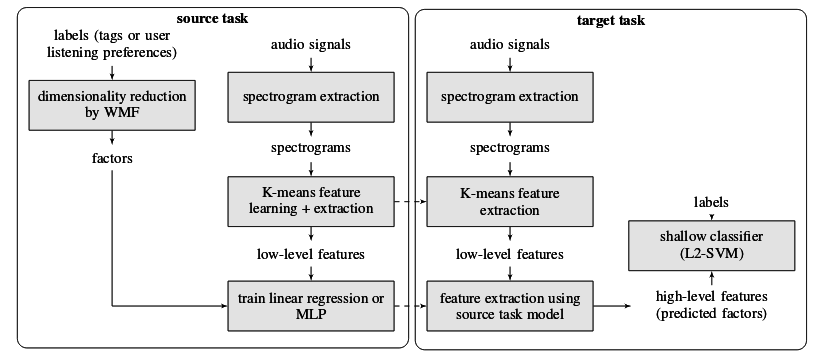
\includegraphics[width=0.95\textwidth]{specLeak1}
\caption{Schematic overview of the workflow of transfer learning}
 \label{fig:transfer learning}
 \end{figure}
\FloatBarrier
\bigskip

\noindent \textbf{Source task}: 
The low-level features from audio spectrograms are learned through unsupervised learning by spherical K-Means. A multi layer perceptron is then stacked to obtain final prediction. So the output from the penultimate layer of MLP are treated as transferable features. To tackle problems created by redundant and sparse labels, dimensionality reduction is done in the label space using PCA. The model is then trained to predict the reduced label representation.
\bigskip

\noindent \textbf{Target task}
Next,  the trained models are used to extract features from other datasets, which are then passed to train shallow classifiers for different but related target tasks. This workflow is visualized in fig[ ] Dashed arrows indicate transfer of the learned feature extractors from the source task to the target task.
\bigskip

\noindent It has been shown that features learned in this fashion work well for auxiliary audio classification tasks on different datasets, consistently outperforming a purely unsupervised feature learning approach.

\subsection{Convolutional Neural Networks}
It can be seen that deep signal processing structures can be realized by stacking multiple shallow architectures. As feature learning was proving to be more efficient than hand crafted features, stacking learnable layers over one another became a hot area of research. Following the success of convolutional neural networks in computer vision [ ] and speech recognition [], experiments were also done for music auto-tagging [] [] []. The idea was to replace the application specific dimension reductions with hierarchy of learnable convolution filters (see \ref{deep learning}) 

\subsubsection{End to end learning of music audio}
As shown in chapter 2, all operations including FFT can be defined in terms of convolutions. In this research they investigate whether it is possible to apply feature learning directly to raw audio signal. The signal was convolved with 3 layers of 1D convolutions followed by two fully connected layers for predicting the tag. Thus, the feature and the classifier was trained in a single pipeline and this was called end to end learning. They compared the end to end learning approach with convolutions from mel-spectrogram on MTT dataset (i.e, retaining STFT). It was found that, discarding STFT hurt the performance. CNN from mel-spectrogram achieved 0.8815 AUC, but on including convolutions on audio signal AUC dropped to 0.8487.     
 
\begin{minipage}[t]{7.5cm}
  \vspace{0pt}  
  \begin{algorithm}[H]
    \caption{CNN(raw audio) [\textbf{0.84}]}
    \begin{algorithmic}[1]
      \Statex \textbf{Input :} $\textbf{a} \in \mathbb{R}^{N}$
      \Statex \textbf{Output :} $Pred \in \mathbb{R}^{L}$ 
      \State $\textbf{C}_{1}  = Log(\textbf{a}\star\textbf{w}_{(256)}^{(256)})$
      \State $\textbf{C}_{2} =  MaxPool(ReLU(\textbf{C}_{1}\star\textbf{w}_{(32)}^{(1)}))$
       \State $\textbf{C}_{3} = MaxPool(ReLU(\textbf{C}_{2}\star\textbf{w}_{(32)}^{(1)}))$
       \State $\textbf{y} = FLATTEN(\textbf{C}_{3})$
       \State $Pred = \sigma(L(\textbf{W}_{2})ReLU(L(\textbf{W}_{1})\textbf{y}))$
   \end{algorithmic}
  \end{algorithm}
\end{minipage}%
\begin{minipage}[t]{7.5cm}
  \vspace{0pt}
  \begin{algorithm}[H]
    \caption{CNN(Mel-Spectrogram) [\textbf{0.88}]}
     \begin{algorithmic}[1]
      \Statex \textbf{Input :} $\textbf{a} \in \mathbb{R}^{N}$
      \Statex \textbf{Output :} $Pred \in \mathbb{R}^{L}$ 
      \State $\textbf{R}  = MEL(||STFT(\textbf{a})||^{2})$
      \State $\textbf{C}_{1} =  MaxPool(ReLU(\textbf{R}\star\textbf{w}_{(32)}^{(1)}))$
       \State $\textbf{C}_{2} = MaxPool(ReLU(\textbf{C}_{1}\star\textbf{w}_{(32)}^{(1)}))$
       \State $\textbf{y} = FLATTEN(\textbf{C}_{2})$
       \State $Pred = \sigma(L(\textbf{W}_{2})ReLU(L(\textbf{W}_{1})\textbf{y}))$
   \end{algorithmic}
  \end{algorithm}
\end{minipage}

\subsubsection{Experimenting musically motivated CNNs}
In the previous section, only 1D convolution with filter sizes directly motivated by hand-crafted methods were tested for comparison. But usually, the convolution operation allows flexibility in choosing the filter sizes. In this research, the authors discuss how convolution filters with different shapes can fit specific musical concepts. 
\begin{figure}[h]
       \begin{subfigure}[b]{0.3\textwidth}
        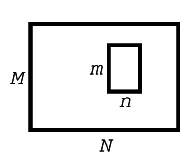
\includegraphics[width=\textwidth]{square}
        \caption{Rectangular filter }
        \label{fig:square}
       \end{subfigure}
	    \begin{subfigure}[b]{0.3\textwidth}
        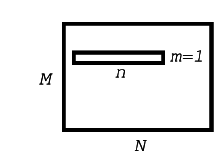
\includegraphics[width=\textwidth]{time}
        \caption{
        Time filter
        }
        \label{fig:time}
       \end{subfigure}
       	    \begin{subfigure}[b]{0.3\textwidth}
        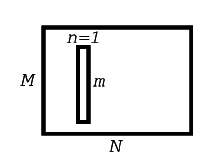
\includegraphics[width=\textwidth]{freq}
        \caption{
        Frequency filter
        }
        \label{fig:freq}
       \end{subfigure}
       \caption{Different Filter sizes}\label{fig:STFT}
\end{figure}
\FloatBarrier
\bigskip 
\noindent \textit{Time filters} can learn temporal cues (Onset, BPM and other rhythmic patterns), while \textit{frequency filters} can differentiate timbre and note. \textit{Rectangular filters} can learn short time sub-bands (Bass, kick, drums) [ ]. However, because of hierarchical nature of deep networks, any filter should be theoretically capable of picking up the relevant cues. It was shown in their experiments that \textit{rectangular filters} or combination of time and frequency filters performed better than using just time / frequency filter. These experiments were however done for a genre classification task.  

\subsubsection{Automatic tagging using deep convolutional neural network}
Different CNN architectures were tested and the proposed model achieves close to state of art performance on MTT dataset (0.894 AUC). The audio samples were down-sampled to 12 KHz and convolutions were started from mel spectrogram (96 bins). They also compared MFCCs, convolutions over STFT and convolutions over Mel-spectrogram and report that the latter performs significantly better.

    \begin{tabular}{ | p{5cm} | l |}
    \hline
    \textbf{Model} & \textbf{AUC} \\ \hline
    STFT $\rightarrow$ CNN &  0.846\\ \hline
    STFT $\rightarrow$ MEL $\rightarrow$ CNN &  \textbf{0.894}\\ \hline
    STFT $\rightarrow$ MEL $\rightarrow$ MFCC &  0.862 \\ \hline
    \hline
    \end{tabular}
    
Also, to exploit the advantage of PCA Whitening proven in [] [], Batch Normalization[] of frequency components is done. That is, data is centred to the batch mean and divided by batch variance. In Batch normalization however, the basis is not switched but the data is \textit{learned} to be scaled and shifted.
\begin{algorithm}
  \caption{$\textbf{\^{X}}$ = BATCHNORM($\textbf{X}$) }\label{Batch norm}
  \begin{algorithmic}[1]
    \Statex \textbf{Input :} $\textbf{X} \in \mathbb{R}^{B \times S \times Q}$, \Comment{$B$ is batch size}
    \Statex \textbf{Output :} $\textbf{\^X} \in \mathbb{R}^{B \times S \times Q}$ 
    \Statex \textbf{Parameters to learn :} $\gamma$ (Scale), $\beta$ (Shift) 
    \State $\bm{\mu}, \bm{\sigma}^{2} = FREQUENCY\_MEAN\_VARIANCE(\textbf{X})$ \Comment{$\bm{\mu},\bm{\sigma}^{2} \in \mathbb{R}^{S}$}
    \For{$i \in \{1,..,B\}$}
     \For{$j \in \{1,..,Q\}$}
       \State $\textbf{X}[i,:,j] \leftarrow \frac{\textbf{X}[i,:,j] - \bm{\mu}}{\sqrt{\bm{\sigma}}^{2} - \epsilon}$
      \EndFor
     \EndFor
     \State $\textbf{\^X} = \gamma\textbf{X} + \beta$
  \end{algorithmic}
\end{algorithm}
\FloatBarrier

\noindent The five layer proposed CNN architecture is shown below. The filters $\textbf{W}$ in each layer are the weights that will be learned. $Spatial\_Bn$ is similar to the normalization algorithm mentioned above, except that the normalization is done along the 1st axis of tensors $\textbf{C}$. $MaxPool_{i,j}$ is a dimensionality reduction done by pooling $(i,j)$ elements along $S$ and $Q$ directions respectively. $Elu$ is an element-wise non-linearity operation described in section (??) 

\begin{algorithm}
  \caption{$\textbf{y}$ = $CHOI\_CNN(\textbf{R})$ }      
  \begin{algorithmic}[1]
   \Statex \textbf{Input :} $\textbf{R} \in \mathbb{R}^{1 \times 96 \times 1366}$
   \Statex \textbf{Output :} $\textbf{y} \in \mathbb{R}^{1024}$ 
   \State $\textbf{R}_{n} = BatchNorm(\textbf{R})$
   \State $\textbf{C}_{1} = \textbf{R}_{n}\star\textbf{W1}_{(32)}^{(1,1)}$ \Comment{$\textbf{W1} \in \mathbb{R}^{32 \times 3 \times 3}, \textbf{C}_{1} \in \mathbb{R}^{32 \times S1 \times Q1}$}
   \State $\textbf{C}_{1} \leftarrow MaxPool_{(2,4)}(Elu(Spatial\_Bn(\textbf{C}_{1})))$ \Comment{$\textbf{C}_{1} \in \mathbb{R}^{32 \times T1 \times W1}$}
      \State $\textbf{C}_{2} = \textbf{C}_{1}\star\textbf{W2}_{(128)}^{(1,1)}$ \Comment{$\textbf{W2} \in \mathbb{R}^{128 \times 3 \times 3}, \textbf{C}_{2} \in \mathbb{R}^{128 \times S2 \times Q2}$}
   \State $\textbf{C}_{2} \leftarrow MaxPool_{(2,4)}(Elu(Spatial\_Bn(\textbf{C}_{2})))$ \Comment{$\textbf{C}_{2} \in \mathbb{R}^{128 \times T2 \times W2}$}
         \State $\textbf{C}_{3} = \textbf{C}_{2}\star\textbf{W3}_{(128)}^{(1,1)}$ \Comment{$\textbf{W3} \in \mathbb{R}^{128 \times 3 \times 3}, \textbf{C}_{3} \in \mathbb{R}^{128 \times S3 \times Q3}$}
   \State $\textbf{C}_{3} \leftarrow MaxPool_{(2,4)}(Elu(Spatial\_Bn(\textbf{C}_{3})))$ \Comment{$\textbf{C}_{3} \in \mathbb{R}^{128 \times T3 \times W3}$}
         \State $\textbf{C}_{4} = \textbf{C}_{3}\star\textbf{W4}_{(192)}^{(1,1)}$ \Comment{$\textbf{W4} \in \mathbb{R}^{192 \times 3 \times 3}, \textbf{C}_{4} \in \mathbb{R}^{192 \times S4 \times Q4}$}
   \State $\textbf{C}_{4} \leftarrow MaxPool_{(2,4)}(Elu(Spatial\_Bn(\textbf{C}_{4})))$ \Comment{$\textbf{C}_{4} \in \mathbb{R}^{192 \times T4 \times W4}$}
         \State $\textbf{C}_{5} = \textbf{C}_{4}\star\textbf{W5}_{(256)}^{(1,1)}$ \Comment{$\textbf{W5} \in \mathbb{R}^{256 \times 3 \times 3}, \textbf{C}_{5} \in \mathbb{R}^{256 \times S5 \times Q5}$}
   \State $\textbf{C}_{5} \leftarrow Elu(Spatial\_Bn(\textbf{C}_{5}))$ 
   \State $\textbf{y} = Flatten(\textbf{C}_{5})$ \Comment{$\textbf{y} \in \mathbb{R}^{1024}$}
  \end{algorithmic}
\end{algorithm}
\FloatBarrier

\noindent The features from convolutions then pass through a fully connected layer of size equalling  number of tags. The authors have then trained this model on MSD dataset and made the weights publicly available.

\section{Model Selection}

In Chapter 2 (sec ??), it was argued that aesthetic discrimination of songs are due to the components of rhythmic patterns that make up the trajectory of a music signal. Then it was shown how MFCCs extract this trajectory information (see ??). In the current literatures discussed above[],[],[], MFCC computations were done on general spectrum where harmonically relation of frequencies are not exploited. Hence the job of separating the rhythmic components is left to the classifier.     

From the literatures elaborated in previous section, it is possible to infer that feature learning achieves better performance than MFCC for multi-label classification task [auto tag, temporal]. As the fully unsupervised feature learning [] performs better than MFCCs, there is an indication that it is possible to get better features than MFCCs irrespective of the size of dataset.
\externaldocument{chapter1}
\chapter{Experiments and Results} % Main chapter title

\label{Chapter4} % For referencing the chapter elsewhere, use\ref{Chapter2} 

The aim of this thesis is to find the optimal algorithm for content-based multi-label classification of music tracks, that can be solved with minimal training data. We are looking for a classifier that can discriminate aesthetics in music, but the public datasets are socially biased and contains only short excerpts. Hence the multi-label classifiers have to be tested on our unbiased target dataset which has full clips. In Chapter 3, the state of art models were reviewed and in section \ref{model}, the short-comings of these algorithms in addressing the problems discussed in Chapter 1 (see \ref{problems}) were pointed out. In this chapter, the experiments that will lead to finding the best algorithm using the components short-listed in \ref{model} will be described.

\section{Dataset and Evaluation}
\label{dataset}
More specific to our task than representing audio is finding a proper dataset of labelled pairs. Recalling that our aim is to identify the aesthetic properties of music from the audio content, a dataset that is free from \textit{audio-semantic} noise is needed. Furthermore, to test \textit{transfer learning}, a large dataset is needed for the \textit{source task} (ref. \ref{transfer}). Popularly used \textit{Million Song Dataset} (MSD) \cite{MSD} contains a cluster of complimentary datasets, most of them annotated with \textit{social tags}. For instance, \textit{Last.fm} which forms a part of MSD contains annotations from users of an online radio application. But such social tags contribute to the \textit{audio-semantic} noise which we want to eliminate. The dataset that is mostly used for evaluating content-based algorithms is \textit{Magna Tag A Tune} dataset \cite{MTT}, where annotations are gathered through a game application that attracts users who are familiar with technical terms related to music. Hence the tags in this dataset are usually clean. Hence this would be a decent choice for our \textit{source task}.

\subsection{Dataset for source task}
\label{source}
The MagnaTagATune dataset consists of 25,856 clips of 29.1-s, 16 kHz-sampled mp3 files with 188 tags. These annotations are gathered from an online game called \textit{Tag a Tune}. A player is partnered up with another random player who cannot be communicated. Both listen to some track, and have to select appropriate tags. Then the players are asked one simple question : "Are we listening to same song?". Answering this correctly will earn them points. This dataset is the largest available that comes close to minimizing the \textit{audio-semantic} noise. However, social factor still plays a role here. This is partly indicated by tag frequency where the most frequent tag is used 4,851 times while the $50^{th}$ most frequent one used 490 times in the training set. We use only the top-50 tags for training from this dataset.  

\subsection{Dataset for target task}
\label{target}
To gather annotations with clean mapping to aesthetic properties, we adopt the most straightforward and costly method - ask someone to listen to songs and tag them. Around 900 songs approximately 5 - 8 min long, were tagged by my supervisor Prof. Paolo Bientinesi in association with Prof. Marco Aluno (Professor of Composition and Theory at University EAFIT, Columbia). Out of 900 songs, 100 are used for validation.  

\subsection{Evaluation metrics}
\label{evaluation}
[TODO]

\section{Experiments}
\label{experiments}
As with any MIR task, the raw audio signal containing amplitude values in time domain is first down sampled and representation parameters are fixed (ref. \ref{stft}). This is because computational cost is heavily affected by the size of the input layers.
\bigskip
 
\noindent \textbf{Sampling Parameters : } Although most of the available audio in digital format are sampled at 44KHz (ref. \ref{sampling}), it is important to note that most of the information lie in the lower range of the spectrum. In \cite{choi_cnn}, a pilot experiment was conducted to demonstrate similar performance with 12KHz and 16KHz for top 50 tags (Recall that MTT clips are already downsampled to 16KHz). Hence we sample all our tracks to 12KHz. 
\bigskip

\noindent Next step is to extract relevant features. General pipeline is \textit{sampling} (ref. \ref{sampling}), \textit{representation} (ref. \ref{stft}), stacks of \textit{dimensionality reduction} (ref. \ref{dimension}) followed by \textit{temporal summarization} (ref. \ref{temporal}). Feature learning can be introduced at different stages. Introducing in earlier stages would require training with huge amount of data. Feature learning on raw sampled signal proved sub-optimal in \cite{EndToEnd}. Same was the case when convolved over STFT frame \cite{choi_cnn}. Convolutions over mel-spectrogram performed better than MFCC in many previous work \cite{choi_cnn}\cite{EndToEnd}. Hence we stick to engineered features until the extraction of mel-spectrogram.  
\bigskip 

\noindent \textbf{Mel-Spectrogram Parameters :}
The signal in the time domain is converted to frequency domain by Short-Time-Fourier-Transform ($STFT$) using Fast-Fourier-Transform(FFT) algorithm. The arguments for doing this were presented in Chapter 2 (ref. \ref{stft}). The parameters for FFT are the size (often referred as FFT Size) and stride (often referred as hop-length) of the window function. FFT size was fixed to 512 (42 ms) and hop-length was fixed to 256. Motivated by the human auditory system, the frequency axis is binned to mel-scale and log of squared STFT coefficients (proportional to loudness) are calculated. In \cite{choi_cnn}, it was stated that 96 mel-bins were optimum.   
\bigskip

\noindent Feature learning over mel-spectrogram still requires large dataset, but our target dataset is small. Hence by questing the effectiveness of feature learning over spectrogram with MFCCs, we decided  to compare both.
\bigskip

\subsection{Experiments with pre-trained CNNs as feature extractor}
\label{pretrained}
In Chapter 2 (ref. \ref{stacked}), it was shown how Convolution Neural Networks (CNN) are motivating to be used as feature extractor for music signal. In Chapter 3 (ref. \ref{convolution}) some of the successful mel-spectrogram convolution architectures trained on MTT dataset showing state-of-art performance were discussed. Now we would like to see if such features extracted through these models can be used for auxiliary tasks. That is to say, the learned CNN parameters (weights) from \textit{source} dataset are used as initialization setting for \textit{target} tasks.    
\bigskip

\noindent The CNN architecture from \cite{choi_cnn} achieves the best AUC score on MTT dataset and hence this architecture is used for feature extraction. The algorithm for their model ($CHOI\_CNN$) is explained in section \ref{convolution} (Algorithm \ref{alg:choicnn}). The input to their CNN was 29.1s mel-spectrogram with representation parameters mentioned above (Thus resulting in 1366 time samples). So for our task, features are extracted every 29.1s and sequentially sent to RNN. The temporal summarization is done by 2 layer \textit{Long Short-Term Memory Recurrent Neural Network} (ref. \ref{rnn}). The RNN module does sequence to one mapping ($Seq2One$) of the input features. This entire model is then trained for 150K iteration on MTT dataset with top 50 tags. Their model was already trained on Million Song Dataset \cite{MSD} with top 50 \textit{Last.fm} tags. We just fine-tune their model on MTT dataset after merging clips from same song. Features of clips from same song are sequentially given as input to RNN with a dropout (ref. \ref{training}) of 0.3 after each layer, which then projects to a fixed sized feature vector. The output of RNN is then passed to a fully connected layer with 50 output units and \textit{sigmoid} activation. ADAM optimizer with \textit{binary-cross-entropy} loss function is used for training. The starting learning rate is $0.001$, decaying at $1^{-8}$ and beta $0.99$ (ref. \ref{training}). Algorithm for $L$ labels is described below and the notations used are consistent with formalisms in Chapter \ref{Chapter2}. The algorithm is implemented in \textit{Torch} [torch] and mel-spectrogram was extracted using \textit{Librosa} [librosa]
\bigskip 

\begin{algorithm}
  \caption{$Pred$ = MODEL($\textbf{a}$) }
  \label{alg:cnnrnn}
  \begin{algorithmic}[1]
    \Statex \textbf{Input :} $\textbf{a} \in \mathbb{R}^{N}$
    \Statex \textbf{Output :} $Pred \in \mathbb{R}^{L}$ 
    \State $\textbf{C} = STFT(\textbf{a})$ \Comment{$\textbf{C} \in \mathbb{C}^{M \times P}$}
    \State $\textbf{Y}_{r} = Log(\textbf{C} \odot \textbf{C})$ \Comment{$\textbf{Y}_{r} \in \mathbb{R}^{M \times P}$}
    \State $\textbf{R} = MEL(\textbf{Y}_{r})$ \Comment{$\textbf{R} \in \mathbb{R}^{96 \times P}$}
    \State $W = floor(\frac{P}{1366})$
    \For{$i \in \{0,..,W\}$}
      \State $\textbf{X} \leftarrow \textbf{R}[:][i:(i+1).1366]$ \Comment{$\textbf{X} \in \mathbb{R}^{96 \times 1366}$}
      \State $\textbf{Y}[i] \leftarrow CHOI\_CNN(\textbf{X})$ \Comment{$\textbf{Y} \in \mathbb{R}^{1024 \times W}$} 
    \EndFor
    \State $\textbf{Y}_{1} = Drop_{(0.3)}(Seq2Seq\_LSTM(\textbf{Y}))$ \Comment{$\textbf{Y}_{1} \in \mathbb{R}^{1024 \times W}$}
    \State $\textbf{y}_{2} = Drop_{(0.3)}(Seq2One\_LSTM(\textbf{Y}_{1}))$ \Comment{$\textbf{y}_{2} \in \mathbb{R}^{1024}$}
    \State $Pred = \sigma(L(\textbf{W})\textbf{y}_{2}))$ \Comment{$\textbf{W} \in \mathbb{R}^{L \times 1024}$}
  \end{algorithmic}
\end{algorithm}
\FloatBarrier

\noindent This CNN model can either be used as a \textit{black-box} feature extractor (That is, weights of the model are not modified while training the \textit{target-task}) or certain layers can be \textit{fine-tuned} (That is, we continue the training on \textit{target-task}). Both the cases are looked separately,
\bigskip

\noindent \textbf{Blackbox CNN + RNN :}\\ 
The weights of CNN trained on the source task are not modified (no fine-tuning). The weights of RNN are also initiazied with those trained on source task. The fully-connected layer in the source task is changed to 65 output units. (i.e 65 labels). The network is trained by back-propagating through the fully connected layer and RNN with \textit{binary-cross entropy} loss function (ref. \ref{training}). The optimization parameters are same as that of \textit{source task}. Training is stopped after 25K iterations, after which the model begins to over-fit. Weighted averaged AUC (WAUC) was \textbf{0.65}
\bigskip

\noindent \textbf{Fine-tune CNN + RNN :}\\
With the same parameter settings, the last layer of CNN was finetuned after 5K iterations. Training was then continued until 25K iterations and WAUC went up to \textbf{0.69}. When last two CNN layers were finetuned WAUC further improved to \textbf{0.71}. Fine-tuning earlier layers proved sub-optimal. 
\bigskip

\noindent This tells us that in the final layers CNN tend to find features specific to task. (Recalling that labels for source and target tasks are different). However, we still do not know if convolutions over mel-spectrogram will be better than MFCCs which is proven to model audio discriminants. Before going there, the effectiveness of RNN should also be questioned. It was hypothesised in Chapter 3 (\ref{model}) that Bag-of-Frames (\ref{clustering}) features using K-Means (which was actually used in \cite{MultiScale} to attain state of art performance) may not be suitable for summarizing features for longer audio. So we test this by replacing RNN with Bag Of Frames (BoF) features.
\bigskip

\noindent \textbf{CNN + BoF :}
The CNN is first finetuned for 10K iterations with algorithm \ref{alg:cnnrnn}. Then 1024 centroids of CNN features are found by unsupervised training on both MTT and our target dataset. This is followed by multi layer perceptron with a hidden layer of 512 units and ReLU activation. Having hidden size of 1024 did not improve the result. WAUC was \textbf{0.67}. The algorithm is described below,

\begin{algorithm}
  \caption{$Pred$ = MODEL($\textbf{a}$) }\label{alg:cnnbow}
  \begin{algorithmic}[1]
    \Statex \textbf{Input :} $\textbf{a} \in \mathbb{R}^{N}$
    \Statex \textbf{Output :} $Pred \in \mathbb{R}^{65}$ 
    \State $\textbf{C} = STFT(\textbf{a})$ \Comment{$\textbf{C} \in \mathbb{C}^{M \times P}$}
    \State $\textbf{Y}_{r} = Log(\textbf{C} \odot \textbf{C})$ \Comment{$\textbf{Y}_{r} \in \mathbb{R}^{M \times P}$}
    \State $\textbf{R} = MEL(\textbf{Y}_{r})$ \Comment{$\textbf{R} \in \mathbb{R}^{96 \times P}$}
    \State $W = floor(\frac{P}{1366})$
    \For{$i \in \{0,..,W\}$}
      \State $\textbf{X} \leftarrow \textbf{R}[:][i:(i+1).1366]$ \Comment{$\textbf{X} \in \mathbb{R}^{96 \times 1366}$}
      \State $\textbf{Y}[i] \leftarrow CHOI\_CNN(\textbf{X})$ \Comment{$\textbf{Y} \in \mathbb{R}^{1024 \times W}$} 
    \EndFor
    \State $\textbf{y}_{1} = BagOfFrames(\textbf{Y},1024)$ \Comment{$\textbf{y}_{1} \in \mathbb{R}^{1024}$}
     \State $Pred = \sigma(L(\textbf{W}_{2})ReLU(L(\textbf{W}_{1})\textbf{y}_{1}))$ \Comment{$\textbf{W}_{2} \in \mathbb{R}^{65 \times 512}, \textbf{W}_{1} \in \mathbb{R}^{512 \times 1024}$}
  \end{algorithmic}
\end{algorithm}
\FloatBarrier
    
\subsection{Experiments with MFCCs as feature extractor}    
\label{mfcc}  
MFCCs are still de-facto standard for classifications on small datasets. If CNNs had to outperform MFCCs, the learned parameters should have to encode discriminants similar to MFCCs. MFCCs are computed by taking discrete-cosine transform on log mel-spectrogram (ref. \ref{basis}). Following the comparison strategies from \cite{choi_cnn}, we retain 30 coefficients, their first and second derivative, resulting in a vector of size 90 for each STFT frame.
\bigskip

\noindent \textbf{MFCC + RNN :}\\
Now, MFCCs from every STFT window is passed in a \textit{30s  Batched sequence} to a Sequence to one LSTM, which results in a projection for every 30s window. These sequence of 30s frames are then passed to another Sequence to One LSTM to get a final projection. This is done because a MFCCs from STFT frame will result in a long sequence and RNNs tend to forget the information in the earlier sequence samples. This network was first trained with MTT dataset before our target dataset. The parameter setting are same as those used while training \textbf{CNN+RNN}. The resulting WAUC was \textbf{0.74}   
\begin{algorithm}
  \caption{$Pred$ = MODEL($\textbf{a}$) }\label{alg:mfccrnn}
  \begin{algorithmic}[1]
    \Statex \textbf{Input :} $\textbf{a} \in \mathbb{R}^{N}$
    \Statex \textbf{Output :} $Pred \in \mathbb{R}^{65}$ 
    \State $\textbf{R} = MFCC(\textbf{a})$ \Comment{$\textbf{R} \in \mathbb{R}^{90 \times P}$}
        \State $W = floor(\frac{P}{1366})$
    \For{$i \in \{0,..,W\}$}
      \State $\textbf{X} \leftarrow \textbf{R}[:][i:(i+1).1366]$ \Comment{$\textbf{X} \in \mathbb{R}^{90 \times 1366}$}
    \State $\textbf{Y}[i] \leftarrow Drop_{(0.3)}(Seq2One\_LSTM(\textbf{X}))$ \Comment{$\textbf{Y} \in \mathbb{R}^{1024 \times W}$}
    \EndFor
    \State $\textbf{y} = Drop_{(0.3)}(Seq2One\_LSTM(\textbf{Y}))$ \Comment{$\textbf{y} \in \mathbb{R}^{1024}$}
    \State $Pred = \sigma(L(\textbf{W})\textbf{y}))$ \Comment{$\textbf{W} \in \mathbb{R}^{65 \times 1024}$}
  \end{algorithmic}
\end{algorithm}
\FloatBarrier

\noindent \textbf{MFCC + BoF :}\\
RNN is repalaced with Bag of Frames features. Now WAUC drops to \textbf{0.62}
\begin{algorithm}
  \caption{$Pred$ = MODEL($\textbf{a}$) }\label{alg:mfccbow}
  \begin{algorithmic}[1]
    \Statex \textbf{Input :} $\textbf{a} \in \mathbb{R}^{N}$
    \Statex \textbf{Output :} $Pred \in \mathbb{R}^{65}$ 
    \State $\textbf{R} = MFCC(\textbf{a})$ \Comment{$\textbf{R} \in \mathbb{R}^{90 \times P}$}
   \State $\textbf{y} = BagOfFrames(\textbf{R},1024)$ \Comment{$\textbf{y} \in \mathbb{R}^{1024}$}
     \State $Pred = \sigma(L(\textbf{W}_{2})ReLU(L(\textbf{W}_{1})\textbf{y}))$ \Comment{$\textbf{W}_{2} \in \mathbb{R}^{65 \times 512}, \textbf{W}_{1} \in \mathbb{R}^{512 \times 1024}$}
  \end{algorithmic}
\end{algorithm}
\FloatBarrier    

\section{Summary of Results}
\label{results}
Summary of results is shown in the table below. It is seen that \textit{transfer learning} of convolutions over mel-spectrogram with architecture in \cite{choi_cnn}  cannot match with MFCCs for small datasets. This indicates that convolutional features from source dataset are more task-specific. It is also seen that \textit{Recurrent Neural Networks} perform better in summarizing features for longer audio. This indicates the existence of rhythmic patterns that discriminate music. 

   \begin{tabular}{ | p{5cm} | l |}
    \hline
    \textbf{Model} & \textbf{AUC} \\ \hline
    Finetune CNN + RNN &  0.71\\ \hline
    CNN + BoF  &  0.67\\ \hline
    MFCC + RNN &  \textbf{0.74} \\ \hline
    MFCC + BoF &  0.62 \\ \hline
    \hline
    \end{tabular}


\externaldocument{chapter1}
\externaldocument{chapter2}
\chapter{Conclusion} % Main chapter title

\label{Chapter5}
The performance of music tagging algorithm will be higher if the extracted features encode the acoustic cues necessary for discriminating the semantics. Supervised feature learning is used to obtain features that could be optimal for our context of music tagging. Convolution and recurrent neural networks were used to induct supervised learning into the feature extraction pipeline. The number of parameters to solve increases as the learning problem becomes deeper and hence more training data is required for convergence. Therefore, in this thesis, transfer learning with models trained on \textit{MagnaTagaTune} dataset were analysed by comparing different levels of fine-tuning on the target dataset. It has been found that fine-tuning entire CNN + RNN on target data performs significantly better than just using black-box CNN. It would be useful to bridge this gap to improve performance, because deep levels of training on our target data, which is small, struggles to out-perform MFCC features.     

\subsubsection{Proposal for improvements}
\begin{itemize}
\setlength\itemsep{0em}
\item Since MFCC performs better than fine-tuned CNNs, it would be worthy to analyse CNN architectures trained on the source data by initializing CNN filters with cosine functions to get richer features. (In chapter 2, section \ref{stacked}, an illustration of MFCC computation as convolution operations was shown)
\item Singular value decomposition of the converged filters at each CNN layer can be performed to see if they are converging to any known mathematical function. If it does, then it would be useful to set those functions as initialization before training.   
\end{itemize}
 


% Appendix A

%\chapter*{Frequently Asked Questions} % Main appendix title

%\label{AppendixA} % For referencing this appendix elsewhere, use \ref{AppendixA}
\begin{appendices}

\chapter{}
\section{Basis Transformation}

Here we discuss only transformation from standard \gls{basis} or Cartesian \gls{basis}.
\bigskip

\noindent The standard \gls{basis} for $\mathbb{R}^{N}$ is the ordered sequence $\textbf{E}_{n} = [\textbf{e}_{1}, \textbf{e}_{2}, ..,\textbf{e}_{n}]$, where $\textbf{e}_{i}$ is a vector with 1 in $\textit{i}^{th}$ place and 0 elsewhere. Any vector $\textbf{x} = [x_{1}, x_{2},...,x_{n}] \in \mathbb{R}^{N}$ can be represented as a \gls{linear combination} of $\textbf{E}_{n}$ as,
\[
\textbf{x} = \displaystyle\sum_{i=1}^{N}x_{i}\textbf{e}_{i} = \textbf{E}_{n}\textbf{x}
\]

\noindent \textbf{Basis transformation} from standard \gls{basis} is defined as representing the same vector $\textbf{x}$ with the new co-ordinates $[y_{1}, y_{2},...,y_{m}]$ in \gls{basis} $\textbf{V} = [\textbf{v}_{1}, \textbf{v}_{2}, ..,\textbf{v}_{m}] \in \textbf{R}^{N \times M} $.
\bigskip

\[
\textbf{x} = \displaystyle\sum_{i=1}^{M}y_{i}\textbf{v}_{i} = \textbf{V}\textbf{y} \qquad \textbf{y} \in \mathbb{R}^{M}
\]
$\textbf{V}$ is also known as \textbf{change of coordinates matrix} (also stated as any matrix whose columns form a \gls{basis}). If $\textbf{V}$ is orthogonal, then $\textbf{V}^{-1} = \textbf{V}^{T}$ and hence $\textbf{y} = \textbf{V}^{T}\textbf{x}$

\section{Convolution}
Only discrete convolutions with finite support are discussed below,

\subsection{1D Convolution}
Convolution of a vector $\textbf{f}$ with filter $\textbf{w}_{k}$ of stride $s$ is defined as, 
\begin{equation}
\textbf{C}(k, i) = \displaystyle\sum_{n=i.s}^{i.s + F}\textbf{f}(n)\textbf{w}_{k}(n-i.s) \qquad \textbf{f} \in \mathbb{R}^{N}, \textbf{w}_{k} \in \mathbb{R}^{F}, \textbf{C} \in \mathbb{R}^{K \times I}
\end{equation}
\[
\textbf{C}(k,i) = \textbf{f}(n)\star\textbf{w}_{k}(n-i.s)
\]
Where:
\begin{itemize}[label=]
    \setlength\itemsep{0em}
    \item $K$ is the number of filters. $k \in {0,1...K-1}$ 
    \item $I$ is the number of contractions. $i \in {0,1...I-1}$
\end{itemize}
\textbf{Short Hand Notation :} 1D Convolution of $\textbf{f}$ with filter $\textbf{w}_{k}$ with stride $s$
\[
\boxed{
\textbf{C}(k,:) = \textbf{f}\star\textbf{w}^{(s)}_{k}
}  
\]

\subsection{2D Convolution}
Convolution of a matrix $\textbf{F}$ with filter $\textbf{W}_{k}$ of row-stride $s$ and column-stride $t$ is defined as, 
\begin{equation}
\textbf{C}(k, j, i) = \displaystyle\sum_{n=i.s}^{i.s + F}\displaystyle\sum_{m=j.t}^{j.t + G}\textbf{F}(m,n):\textbf{W}_{k}(m-j.t, n-i.s) \qquad \textbf{F} \in \mathbb{R}^{M \times N}, \textbf{W}_{k} \in \mathbb{R}^{G \times F}, \textbf{C} \in \mathbb{R}^{K \times J \times I}
\end{equation}
\[
\textbf{C}(k,j,i) = \textbf{F}(m,n)\star\textbf{W}_{k}(m-j.t, n-i.s)
\]
\textbf{Short Hand Notation :} 2D Convolution of $\textbf{F}$ with filter $\textbf{W}_{k}$ with row-stride $s$ and column-stride $t$
\[
\boxed{
\textbf{C}(k,:,;) = \textbf{F}\star\textbf{W}^{(s,t)}_{k}
}  
\]

\end{appendices}

% Appendix A

%\chapter*{Frequently Asked Questions} % Main appendix title

%\label{AppendixA} % For referencing this appendix elsewhere, use \ref{AppendixA}
\begin{appendices}

\chapter{Experiments}
\section{Validation Tags}
The list of tags and it's number of occurrences in the validation set.\\
\\
\begin{tabular}{| p{.05\textwidth} | p{.20\textwidth} | p{.05\textwidth}|}
\hline
\textbf{No.} & \textbf{Tag} & \textbf{Freq}\\
\hline
1 & down beat & 3\\
\hline
2 & blip & 3 \\
\hline
3 & bass & 39 \\
\hline
4 & deep & 34 \\
\hline
5 & dark & 4\\
\hline
6 & kick & 33\\
\hline
7 & tight & 9\\
\hline
8 & bass lead & 33\\
\hline
9 & empty & 7\\
\hline
10 & tiro & 5\\
\hline
11 & female & 51\\
\hline
12 & house & 59\\
\hline
13 & happy & 4\\
\hline
14 & piano & 11\\
\hline
15 & male & 19\\
\hline
16 & spoken & 7 \\
\hline
17 & aggressive & 8\\
\hline
18 & tztz & 31\\
\hline
19 & disco & 8\\
\hline
20 & chic & 3\\
\hline
21 & melody & 11\\
\hline
\end{tabular}
\quad
\begin{tabular}{| p{.05\textwidth} | p{.20\textwidth} | p{.05\textwidth}|}
\hline
\textbf{No.} & \textbf{Tag} & \textbf{Freq}\\
\hline
22 & jazzy & 5\\
\hline
23 & drums & 4\\
\hline
24 & train & 4\\
\hline
25 & trip & 2\\
\hline
26 & soulful & 27\\
\hline
27 & unzug & 12\\
\hline
28 & song & 32\\
\hline
29 & steady & 12\\
\hline
30 & slow & 8\\
\hline
31 & loopy & 4\\
\hline
32 & volvo & 11\\
\hline
33 & open & 7\\
\hline
34 & strings & 18\\
\hline
35 & techno & 5\\
\hline
36 & tribal & 3\\
\hline
37 & electro & 4\\
\hline
38 & 1 by 2 & 5\\
\hline
39 & flute & 4\\
\hline
40 & gay & 3\\
\hline
41 & gentle & 5\\
\hline
42 & mellow & 4\\
\hline
\end{tabular}
\quad
\begin{tabular}{| p{.05\textwidth} | p{.20\textwidth} | p{.05\textwidth}|}
\hline
\textbf{No.} & \textbf{Tag} & \textbf{Freq}\\
\hline
43 & soft & 2\\
\hline
44 & rough & 2\\
\hline
45 & energy & 8\\
\hline
46 & voices & 3\\
\hline
47 & get down & 6\\
\hline
48 & warm & 4\\
\hline
49 & elegant & 4\\
\hline
50 & funkyg & 6\\
\hline
51 & upbeat & 6\\
\hline
52 & hypnotic & 5\\
\hline 
53 & choir & 3\\
\hline
54 & scary & 3\\
\hline 
55 & horns & 2\\
\hline
56 & drama & 8\\
\hline
57 & space & 6\\
\hline
58 & ethereal & 6\\
\hline
59 & silly & 5\\
\hline
60 & effects & 2\\
\hline
61 & epic & 4\\
\hline
62 & keys & 4\\
\hline
63 & fast & 4\\
\hline
\end{tabular}
\clearpage

\section{Validation Set}
\label{validationset}
\begin{longtable}{| p{.05\textwidth} | p{.95\textwidth} |}
\hline 
1 & v{\_}Marie St James - Closer I Get \\
\hline
2 & v{\_}Degrees Of Motion - Do You Want It Right Now (Extended Club Mix) \\
\hline
3 & v{\_}Alison Limerick - Where Love Lives (Sauna Mix) \\
\hline
4 & v{\_}Soldiers Of Twilight - Believe (Extended) \\
\hline
5 & v{\_}Dj Spiller - Groovejet (If This Ain't Love) (Spiller's Radio Edit) \\
\hline
6 & Soul Providers - Rise (Ricky Montanari {\&} Stefano Greppi Dark Vocal Mix) \\
\hline
7 & v{\_}Filippo Naugthy Moscatello - Final Signal \\
\hline
8 & v{\_}Aaron-Carl - Dance Naked (Soulman's Eviction Loops) \\
\hline
9 & v{\_}Basement Jaxx - Rendez-Vu (All U Crazies) \\
\hline
10 & v{\_}Deep Dish - My Only Sin \\
\hline
11 & v{\_}St Etienne - Only Love Can Break Your Heart (MAW Dub) \\
\hline
12 & v{\_}Mondo Grosso - Star Suite (Shelter Dub) \\
\hline
13 & v{\_}Brother Of Soul - Ife Bobowa \\
\hline
14 & Malena Perez - Cool Lil Thing (Alix Alvarez dub)\\
\hline
15 & v{\_}Big Moses ft Kenny Bobian - Brighter Days (Original Mix)\\
\hline
16 & v{\_}The Product G{\&}B ft Carlos Santana - Dirty Dancing (Robbie Rivera's Tribal Sessions Sub)\\
\hline
17 & v{\_}NSK Tune - Out Of My Mind (NR Main Dub)\\
\hline
18 & v{\_}Johnick - The Captain\\
\hline
19 & v{\_}Mongobonix - Mas-Pito \\
\hline
20 & v{\_}Basement Jaxx - Rendez-Vu (Radio Edit)\\
\hline
21 & v{\_}Mang'e Le Funk - I Still Want You\\
\hline
22 & LUPO - Hell Or Heaven (Extended Mix)\\
\hline
23 & v{\_}Cevin Fisher - Music Saved My Life (Freezy Jam Mix)\\
\hline
24 & v{\_}Capricorn - Love In London (2001 Mix)\\
\hline 
25 & v{\_}Didier Sinclair - Lovely Flight (Dj Chris Pi Airlines Mix)\\
\hline
26 & v{\_}Africanism - Bisou Sucre\\
\hline
27 & v{\_}Freestyle Orchestra - Twi-Lite (K-Dope Twi-Lite)\\
\hline
28 & v{\_}D.J Spen - Da Changez\\
\hline
29 & v{\_}Men From The Nile - Watch Them Come\\
\hline
30 & v{\_}Deepswing - In The Music (Original Version)\\
\hline
31 & Simone - Hey Fellas (Morel's Gospel Mix)\\
\hline
32 & v{\_}Liquid Measures ft Jocelyn Brown - Take Me Up (Pasta Boys club remix)\\
\hline
33 & v{\_}Jaydee - Plastic Dreams (Morales Club Mix)\\
\hline
34 & v{\_}H20 ft Billie - Take Me Higher (Original Mix)\\
\hline
35 & v{\_}Clivilles {\&} Cole - A Deeper Love (A Deeper Feeling Mix)\\
\hline
36 & v{\_}Confession - I Found My Love (Club Mix A)\\
\hline
37 & v{\_}Discorosso - Discorosso (Kama Kama Vrs.No.1)\\
\hline 
38 & v{\_}Depeche Mode - I Feel Loved (Danny Tenaglia's Labor of Love Instrumental)\\
\hline
39 & v{\_}Djum Djum - Difference (Sagwa Mix)\\
\hline
40 & v{\_}Coco Steel {\&} Lovebomb - Feel It (Vox Mix)\\
\hline
41 & v{\_}Coco Steel {\&} Lovebomb - Feel It (Version Mix)\\
\hline
42 & v{\_}Robbie Rivera - Feel This (Robbie Rivera's Tribal Sessions Mix)\\
\hline
43 & v{\_}Paperclip People - Throw\\
\hline
44 & v{\_}MAW - Unreleased Project (Clouds)\\
\hline
45 & v{\_}D.J Spen - Back When\\
\hline
46 & v{\_}E-Smoove - Be With You (Vocal Vibes)\\
\hline
47 & v{\_}Soul Vision - Don't Stop (Edit)\\
\hline 
48 & v{\_}Lil' Louis {\&} The World - Club Lonely (DJ Pierre's Afro Club Mix)\\
\hline
49 & v{\_}Meli'sa Morgan - Still In Love With You (Still In Love Mix)\\
\hline
50 & v{\_}Rachid - Pride (Album Version)\\
\hline
51 & v{\_}Metro Area - Strut\\
\hline
52 & v{\_}Mekon ft Mark Almond - Please Stay (Bertrand Burgalat's Vocal Remix)\\
\hline
53 & v{\_}Massive Attack - Unfinished Sympathy (Paul Oakenfold Mix)\\
\hline
54 & v{\_}Interfront - Bases Mix R-5\\
\hline
55 & v{\_}Interfront - Mathausen\\
\hline 
56 & v{\_}Interfront - Bonus Beats Strange\\
\hline
57 & v{\_}Future Sound Of London - Papua New Guinea (Qube Mix)\\
\hline 
58 & v{\_}Junior Sanchez - N.A.S.T.Y\\
\hline
59 & v{\_}Full Intention pres Hustle Espanol - (Do The) Spanish Hustle (Dub Mix)\\
\hline
60 & v{\_}Brother Of Soul - Celebration Of Life\\
\hline
61 & v{\_}Gat Decor - Passion (D.Emerson Edit)\\
\hline 
62 & v{\_}Paperclip People - Remake Uno\\
\hline 
63 & v{\_}KenLou 3 - What A Sensation (Sensational Beats)\\
\hline
64 & v{\_}Chiapet - Tick Tock (Apocalypse Now Mix)\\
\hline
65 & v{\_}Aaron-Carl - Dance Naked (C{\&}M Balearic Drama Remix)\\
\hline
66 & v{\_}Starchaser - Jambe Myth (Dsnny Jc vs Speed City Mix)\\
\hline
67 & v{\_}Lil' Devious - Come Home (Dave Clarke Remix)\\
\hline 
68 & v{\_}Bob Marley vs Funkstar De Luxe - Sun Is Shining (ATB Club Mix)\\
\hline
69 & v{\_}Cricco Castelli - Life Has Changed\\
\hline
70 & v{\_}Sandy Rivera - Love For Free\\
\hline
71 & Martha Wash - Leave a Light On\\
\hline
72 & v{\_}Lil' Louis {\&} The World - Club Lonely (Bellbottoms {\&} Platforms Mix)\\
\hline
73 & v{\_}Liquid Woman - Come And Go With Me (Anthem Radio Edit)\\
\hline
74 & v{\_}Age Of Love - The Age Of Love (Sign Of The Time Mix)\\
\hline
75 & v{\_}Interfront - Strange Instru\\
\hline
76 & v{\_}Sonique - Feels So Good (En-Motion Remix)\\
\hline
77 & v{\_}Robert Owens - I'll Be Your Friend (Dead Zone)\\
\hline
78 & v{\_}Crystal Waters - Gypsy Woman (Basement Boys 'Strip To The Bone' Mix)\\
\hline
79 & v{\_}Daft Punk - Around The World (Kenlou Mix)\\
\hline
90 & v{\_}Those Guys - Sierra Leone (Main)\\
\hline
81 & v{\_}Kerri Chandler - Atmosphere (Kerri's Foundation Dub)\\
\hline
82 & v{\_}Rui Da Silva - Touch Me (Peace Division Mix)\\
\hline
83 & v{\_}Cottage Alert - Lost Love (Original Demo Cut)\\
\hline
84 & v{\_}Black Masses - Wonderful Person (Wonderful Brazil Dub)\\
\hline
85 & Basil - City Streets (Kerri Chandler Kaoz On City Streets)\\
\hline
86 & v{\_}Africanism - The Dragon\\
\hline
87 & v{\_}Black Science Orchestra - Keep On Keepin' On (Spen {\&} Karisma's Deepah Dub)\\
\hline
88 & v{\_}The Rolling Stones - Saint Of Me (Deep Dish Grunge Garage Dub)\\
\hline
89 & v{\_}Chez Damier - Can You Feel It (Vocal Club Mix)\\
\hline 
90 & v{\_}Armand van Helden - Entra Mi Casa (Original Long Version)\\
\hline
91 & Jamie Lewis ft Michael Watford - For You (Moodbangers Mix)\\
\hline 
92 & KC Flightt vs Funky Junction - Voices (Pete Heller Main Mix)\\
\hline
93 & v{\_}Toni Braxton - Spanish Guitar (Joe Claussel Dub)\\
\hline 
94 & v{\_}Backroom Congregation - Sunday Morning (WMC 98 Instrumental)\\
\hline
95 & Una Mas - I Will Follow You (Full Intention Club Mix)\\
\hline
96 & v{\_}Modjo - No More Tears (Highpass vs Triple X Remix)\\
\hline
97 & v{\_}Massive Attack - Unfinished Sympathy\\
\hline
98 & v{\_}Bob Sinclair - New York City Music\\
\hline
99 & Kimara Lovelace - I Luv You More (Sean McCabe Demo Mix)\\
\hline
100 & v{\_}The Black Science Orchestra - Sunshine (Sunset Vocal)\\
\hline
\end{longtable}

\end{appendices}

%\chapter{Introduction}
%
%\section{Related work}
%
%Use of references: \cite{BTO,Eigen3}
%
%\section{Outline of the thesis}
%
%\chapter{Chapter title}
%
%\chapter{Experimental results}
%
%\chapter{Conclusions and future work}


%\printbibliography[
%heading=bibintoc,
%title={Bibliography}
%]
 
\printglossaries
\chapter*{Bibliography}
\addcontentsline{toc}{chapter}{Bibliography}
\printbibliography[type={inproceedings},title={Proceedings},heading=subbibliography]
\printbibliography[type={article},title={Articles},heading=subbibliography]
\printbibliography[keyword={preprint},title={Pre-Prints},heading=subbibliography]
\printbibliography[type={book},title={Books},heading=subbibliography]
\printbibliography[type={misc},title={Misc},heading=subbibliography]

\end{document}
